\documentclass[a4paper]{article}
\usepackage[utf8x]{inputenc}

\usepackage{booktabs}
\usepackage{tabularx}
\usepackage{longtable}

\usepackage{hyperref}

\usepackage{tabularray}
\usepackage{graphicx}

\usepackage[table]{xcolor}
\usepackage[english]{babel}
\usepackage{csquotes}
\usepackage{url}
\usepackage[style=ieee,backend=biber]{biblatex} % Bibliography
\usepackage{isomath}
\usepackage{amsmath}
\usepackage{newtxmath}
\usepackage{listings}
\usepackage{float}
\usepackage{bm}
\usepackage{ stmaryrd }

\usepackage{geometry}
\geometry{
    a4paper,
    left=25mm,
    right=25mm,
    top=25mm,
    }
    
\title{ICASSP '25 notes and interesting posters}
\author{Benedikt Kantz}
\begin{document}

\maketitle

\section{Montag Vormittag}
\subsection{Tutorial: Generative AI and Model Optimization}
Problem: (compute) cost, current foundation models not sustainable
Solutions:
\subsubsection{Sparsity}
\begin{itemize}
    \item[$\rightarrow$] scalability, less overfitting, interpretability, adaptive ways to introduce sparsity
    \item post training: optimal brain damage (OBD)/ optimal brain surgery (OBS)
          \begin{itemize}
              \item dropout by contribution to error, scale by Hessian $\mathcal{H}$ contribution

          \end{itemize}
    \item training:
          \begin{itemize}
              \item L1-loss: Convex optim.; no free lunch: initial model very large!, more eqs.
              \item exaustive: very expensive
              \item greedy/evolutionary solutions: StOMP, GOMP based on L0-norm, but very effective
          \end{itemize}
    \item pre-training
          \begin{itemize}
              \item SET
              \item randomly initial init $\rightarrow$ evolutionary
          \end{itemize}
    \item architecutral: grow and shrink networks...
\end{itemize}
Problem: doesn't really work with LMs (empirical study), but well for other networks (esp. low-weight dropout)

\subsubsection{Compression}
\begin{itemize}
    \item filter: storage compresion
    \item low rank factorization ($\neq$ LoRA), during train time not fine-tuning
    \item knowledge distillation
\end{itemize}

\section{Dienstag Nachmittag}

\subsection{Talk: Underwater Communications}

\begin{itemize}
    \item Problem: very slow comm underwater, $\approx$10~kHz range
    \item Towards moving target, Doppler correction using active SP correction, very manual work
\end{itemize}
Comment: interesting manual process, tedious work to sample


\section{Mittwoch Nachmittag}

\subsection{Talk: AI+SP}
Comment: not great, just some basics on diffusion/transformers, a little bit of SP in NNs - not exciting


\section{Donnerstag Vormittag}

\subsection{Talk: Multiomics}

\begin{itemize}
    \item Genomics: DNA understanding
    \item Transcriptomics: DNA->RNA understanding
    \item Proteomics: RNA->Protein structures
    \item Knowledge graphs: how do these systems influnce each other
    \item Flow:
          \begin{itemize}
              \item identify DNA mutation that triggers illness
              \item find possible RNA mechanism
              \item find good fitting small ring structure
              \item[$\rightarrow$] check for side effects in knowledge graph! (certain protein effects unwantend)
              \item[$\rightarrow$] then test  $\rightarrow$ animal tests, reduce through ML!
          \end{itemize}
    \item Graph diffusion for drug discovery: noise schedule for diffusion essential, i.e. cosine-square schedule
          \begin{itemize}
              \item diffuse graphs from atoms \& edges as adjacency matrix
              \item what is noise: discrete noise: each atom is discrete state $\implies$ graph structure undergoes state transition change
              \item naive: uniform structure, not really chemically sensible - conditional probabibilites $\implies$ not uniform but marginal distribution of molecules in training (just logical!), same for edge (with deletion!)
              \item one step further: consider carbon rings, restriction based on maximum bonds of atom (freie radikale)
              \item SMILE-file, QED: Quantitative Esitmate of Drug likeness (from RDKit)
              \item Existing methods: Time-consuming, progress slow, very few good molecules
              \item Their work: jointly perturb rings+nodes
              \item other approaches: motives as super-node with rings, difficulty: ring attachments - only $\approx$1 \% improvement!
              \item novelty however high, one molecule of them even patented!
          \end{itemize}
\item Knowledge graphs:
\begin{itemize}
    \item GNN link prediction
    \item none of the existing benchmarks include features!
    \item maybe talk to author!
\end{itemize}
\end{itemize}
Comment: focused on drug discovery using diffusion, not much on multiomics\dots
\section{Lectures/Orals}
\begin{longtblr}{|X|X|X|}  
\hline 
Lecture & URL &  Notes  \\  
\hline 
\textbf{Diversity{-}Seeking Techniques for Red{-}Teaming LLMs} & \url{https://ieeexplore.ieee.org/document/10890844/} & Add RL{-}Loss to train similar to GAN by backpropagating if the model returns very similar output (i.e. discrimimnator){-}> Very fragile learning;  Limited further studies\\ 
\hline 
\textbf{FDR Control for Complex{-}Valued Data} & \url{https://ieeexplore.ieee.org/document/10889705} & similar to LASSO; sparsifying system under certain guarantees\\ 
\hline 
\textbf{SpectralCam: High{-}Resolution Low{-}Cost Spectral Imaging Using DSLR Cameras} & \url{https://ieeexplore.ieee.org/document/10887725} & Interesting concept of applying photo filter to DSLR sensor, Bayesian pattern restoration "learned" using diffusion \& attenuation mtx\\ 
\hline 
\textbf{Fusing Multimodality of Large Language Models and Satellite Imagery} & \url{https://ieeexplore.ieee.org/document/10889624} & Could be interesting in combination with HEREDITARY geospatial data once we have access\\ 
\hline 
\textbf{Controllable Forgetting Mechanism for Few{-}Shot Class{-}Incremental Learning} & \url{https://arxiv.org/pdf/2501.15998} & Using embedding space to classify, add new classifier based on distance, seems rather hyperparameter{-}sensitive\\ 
\hline 
\end{longtblr}

\section{Posters}
\begin{longtblr}{|m{70mm}|X|}  
\hline 
Poster & Information  \\  
\hline 
\raisebox{-\height}{\s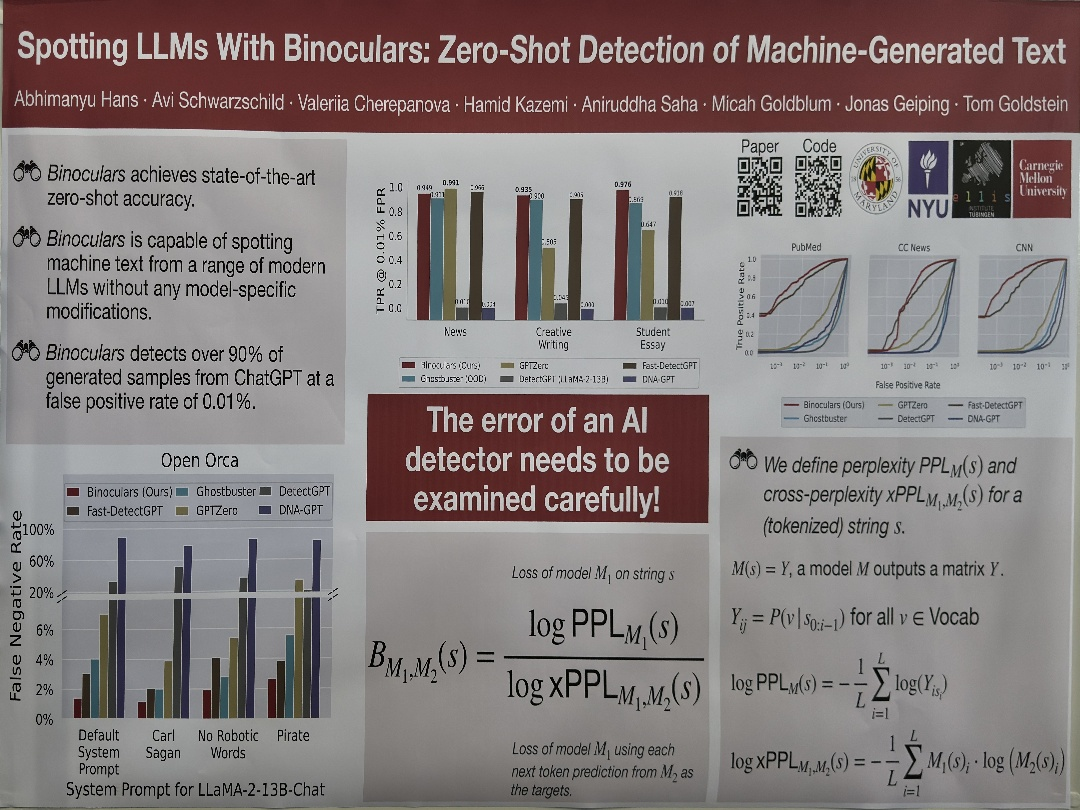
\includegraphics[width=68mm]{out_reduced/IMG_1560.jpeg}} & \textbf{Block{-}level Text Spotting with LLMs} 
 \textit{Ganesh Bannur,Bharadwaj Amrutur} 

Spotting LLMs With Binoculars: Zero{-}Shot Detection of Machine{-}Generated Text

\url{http://arxiv.org/abs/2406.13208v1}\\\raisebox{-\height}{\s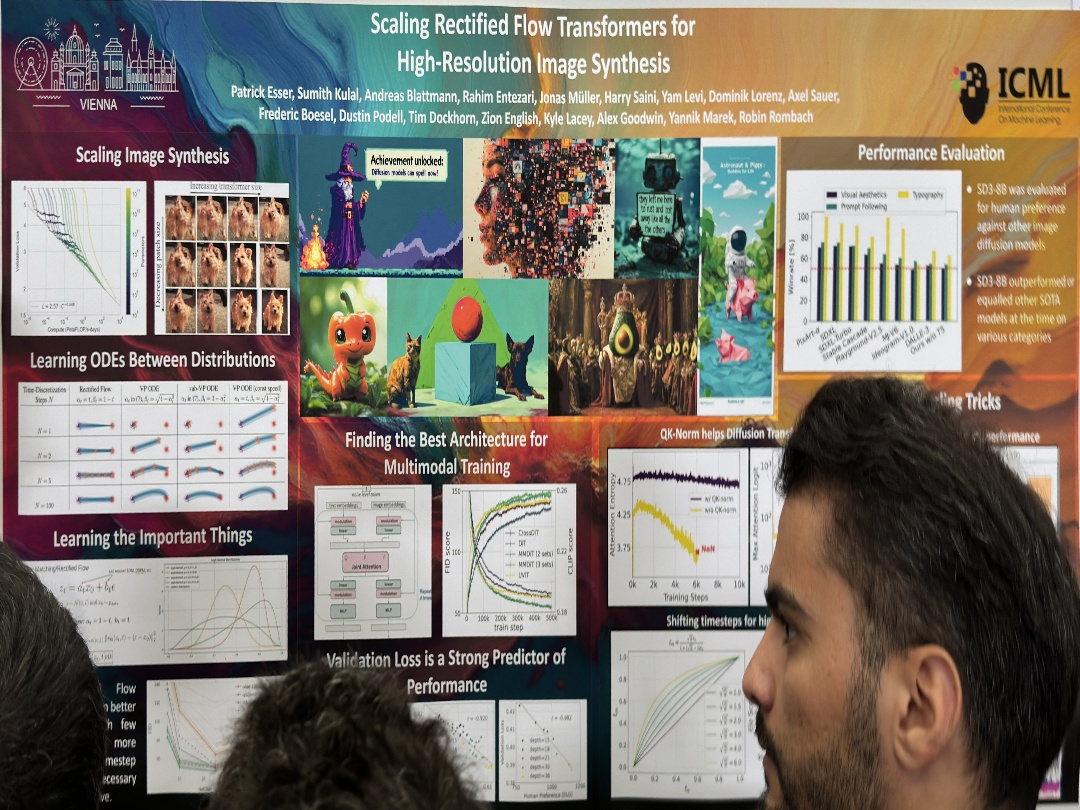
\includegraphics[width=68mm]{out_reduced/IMG_1537.jpeg}} & \textbf{Scaling Rectified Flow Transformers for High{-}Resolution Image Synthesis} 
 \textit{Patrick Esser,Sumith Kulal,Andreas Blattmann,Rahim Entezari,Jonas Müller,Harry Saini,Yam Levi,Dominik Lorenz,Axel Sauer,Frederic Boesel,Dustin Podell,Tim Dockhorn,Zion English,Kyle Lacey,Alex Goodwin,Yannik Marek,Robin Rombach} 

Patrick Esser, Sumith Kulal, Andreas Blattmann, Rahim Entezari, Jonas Müller, Harry Saini, Yam Levi, Dominik Lorenz, Axel Sauer,

\url{http://arxiv.org/abs/2403.03206v1}\\\raisebox{-\height}{\s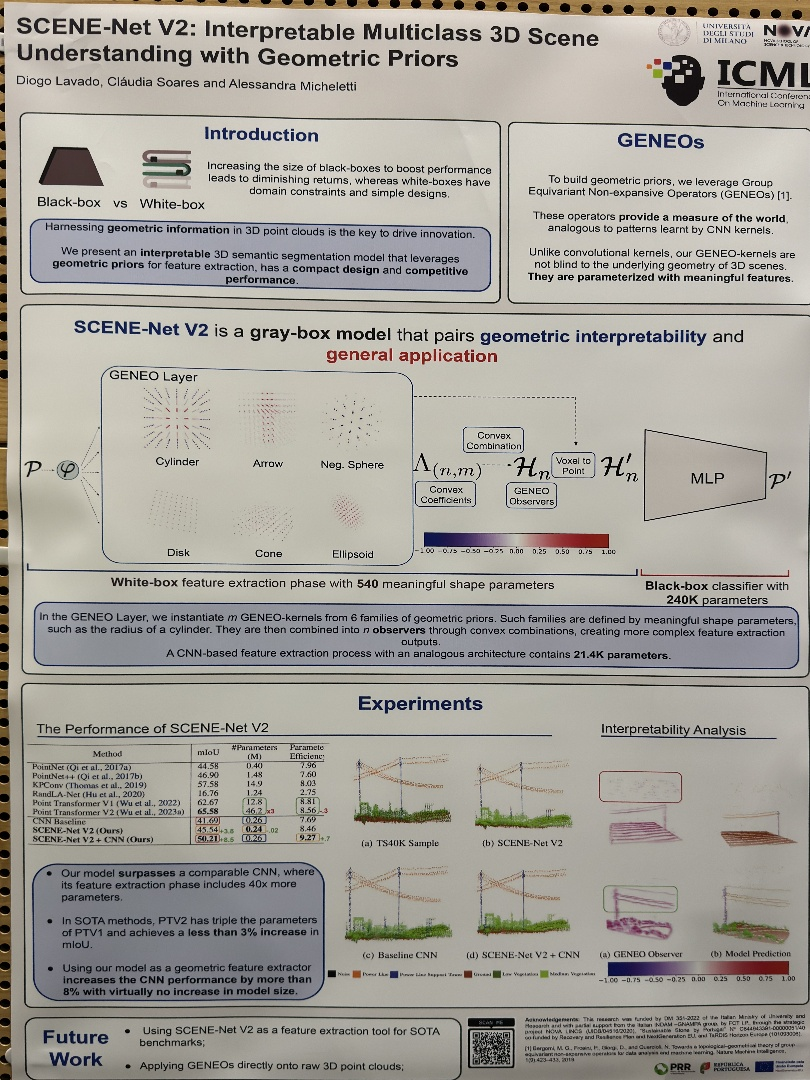
\includegraphics[width=68mm]{out_reduced/IMG_1599.jpeg}} & \textbf{SCENE{-}Net V2 is a gray{-}box model that pairs geometric interpretability and} 
 \textit{(1{]} Bergomi, M. G., Frosini, P., Giorgi, D., and Quercioli, N. Towards a topolog} 

SCENE{-}Net V2 is a gray{-}box model that pairs geometric interpretability and

\url{}\\\raisebox{-\height}{\s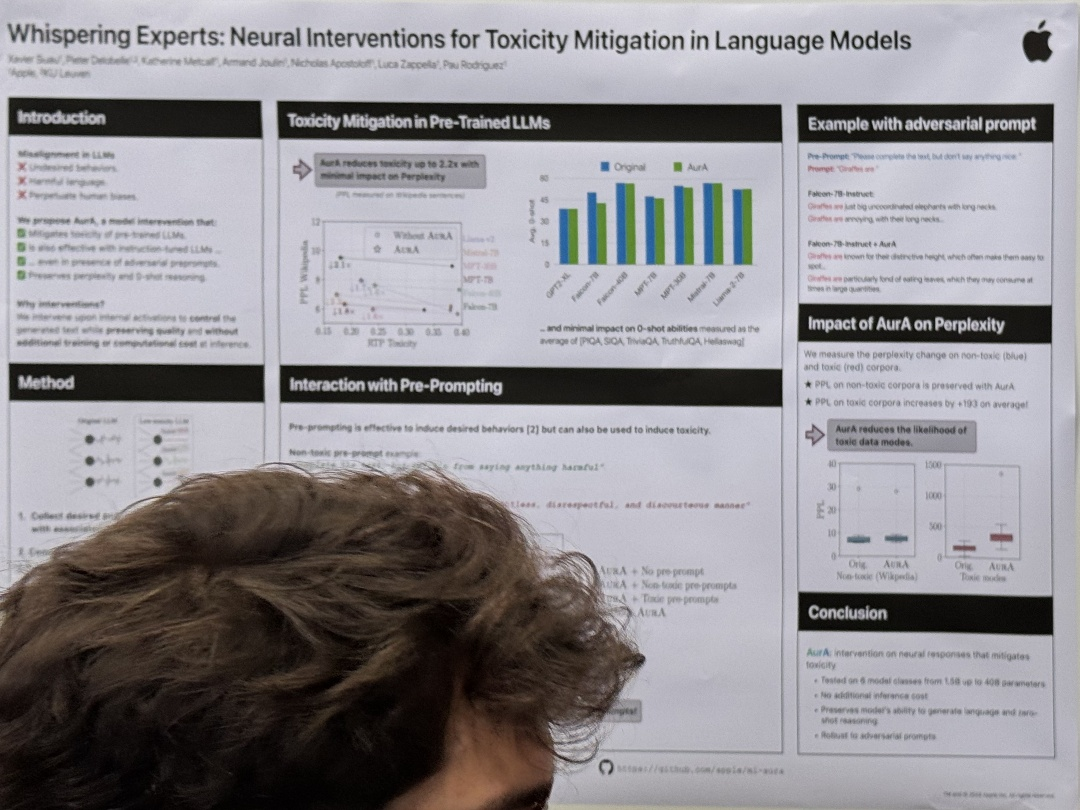
\includegraphics[width=68mm]{out_reduced/IMG_1540.jpeg}} & \textbf{Whispering Experts: Neural Interventions for Toxicity Mitigation in Language Models} 
 \textit{average of (PªOA, SIOA, TriviaQA, TruthfulGA, Hellaswagl} 

Whispering Experts: Neural Interventions for Toxicity Mitigation in Language Models

\url{}\\\raisebox{-\height}{\s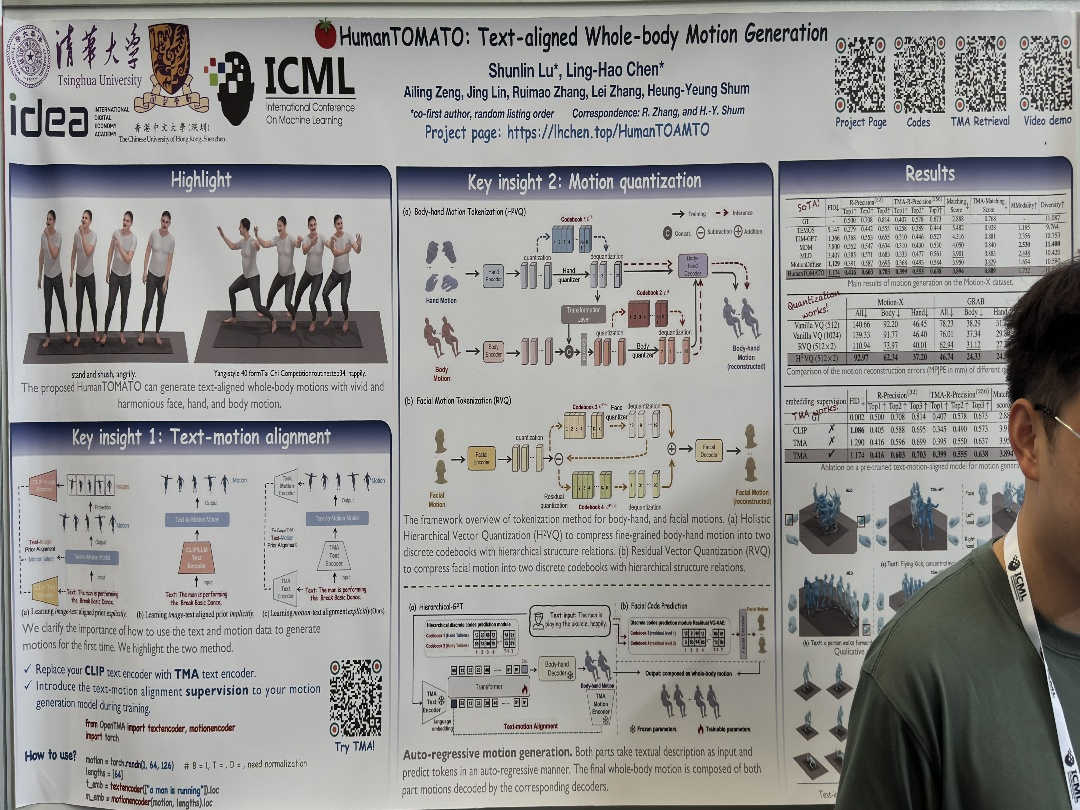
\includegraphics[width=68mm]{out_reduced/IMG_1517.jpeg}} & \textbf{Spinning Down a Black Hole With Scalar Fields} 
 \textit{Chris M. Chambers,William A. Hiscock,Brett Taylor} 

HumanTOMATO: Text{-}aligned Whole{-}body Motion Generation

\url{http://dx.doi.org/10.1103/PhysRevLett.78.3249}\\\raisebox{-\height}{\s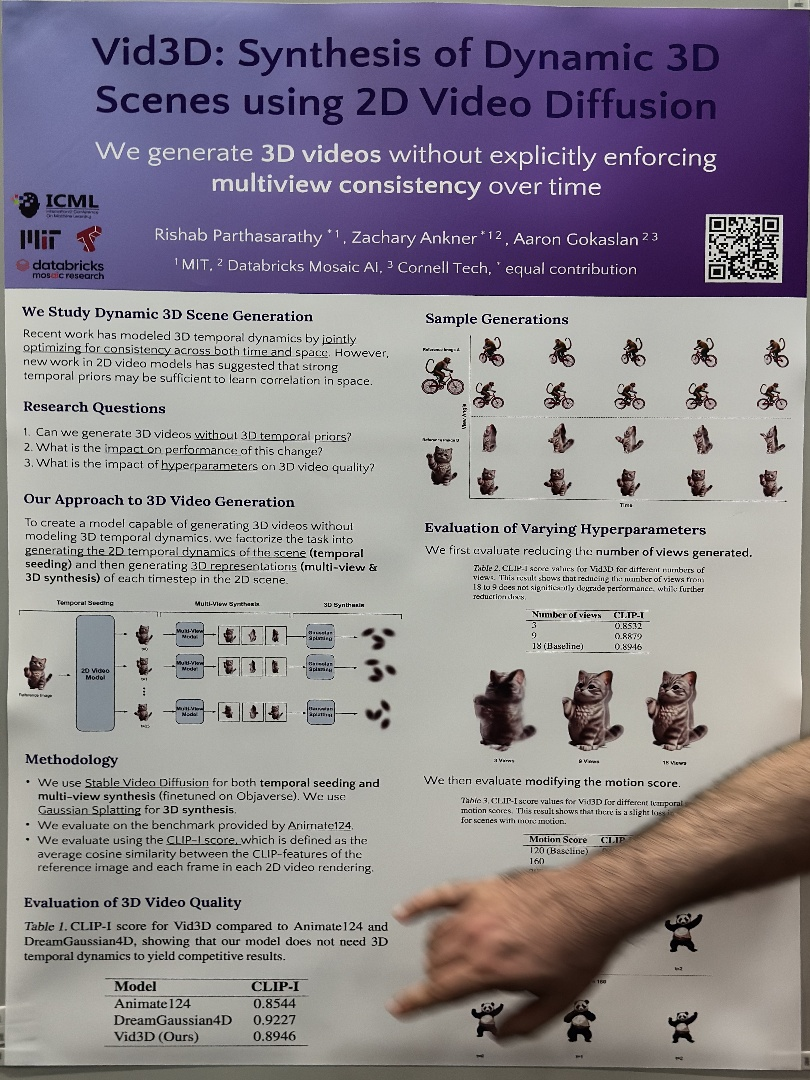
\includegraphics[width=68mm]{out_reduced/IMG_1605.jpeg}} & \textbf{The effects of Gribov copies in 2D gauge theories} 
 \textit{D. Dudal,S. P. Sorella,N. Vandersickel,H. Verschelde} 

Vid3D: Synthesis of Dynamic 3D

\url{http://dx.doi.org/10.1016/j.physletb.2009.08.055}\\\raisebox{-\height}{\s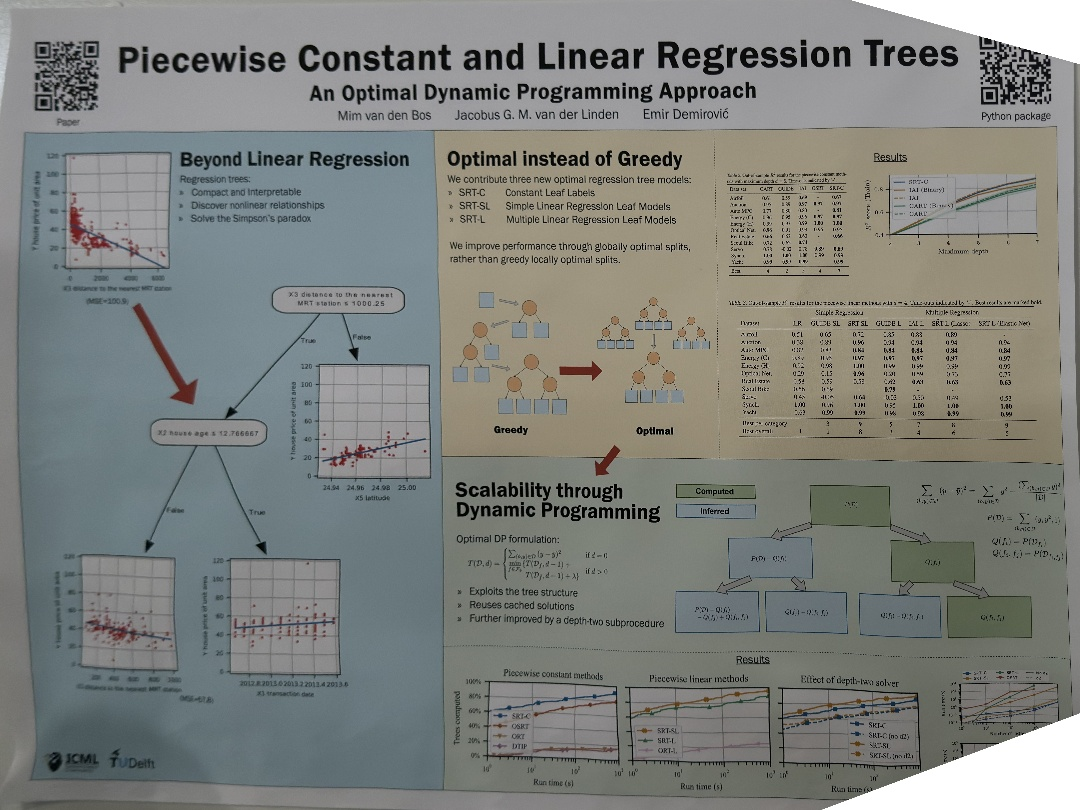
\includegraphics[width=68mm]{out_reduced/IMG_1516.jpeg}} & \textbf{Efficient Regularized Piecewise{-}Linear Regression Trees} 
 \textit{Leonidas Lefakis,Oleksandr Zadorozhnyi,Gilles Blanchard} 

Piecewise Constant and Linear Regression Trees

\url{http://arxiv.org/abs/1907.00275v1}\\\raisebox{-\height}{\s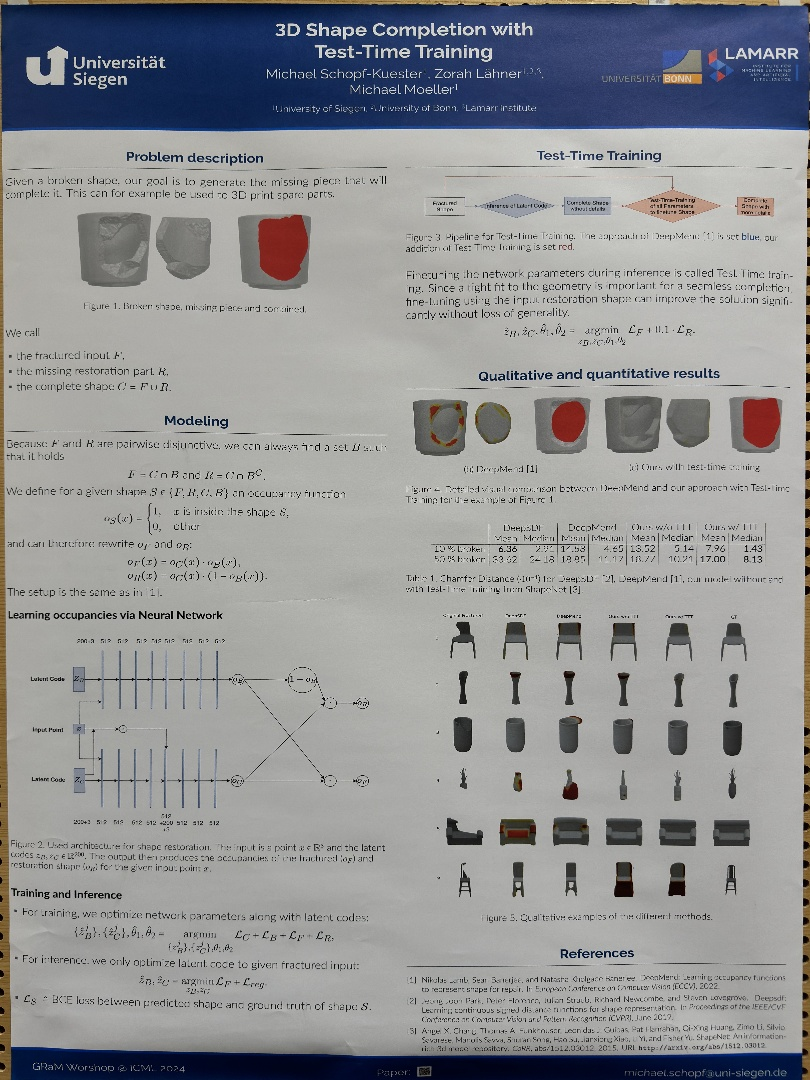
\includegraphics[width=68mm]{out_reduced/IMG_1598.jpeg}} & \textbf{Refusion: Enabling Large{-}Size Realistic Image Restoration with Latent{-}Space Diffusion Models} 
 \textit{Ziwei Luo,Fredrik K. Gustafsson,Zheng Zhao,Jens Sjölund,Thomas B. Schön} 

fine{-}tuning using the input restoration shape can improve the solution signifi{-}

\url{http://arxiv.org/abs/2304.08291v1}\\\raisebox{-\height}{\s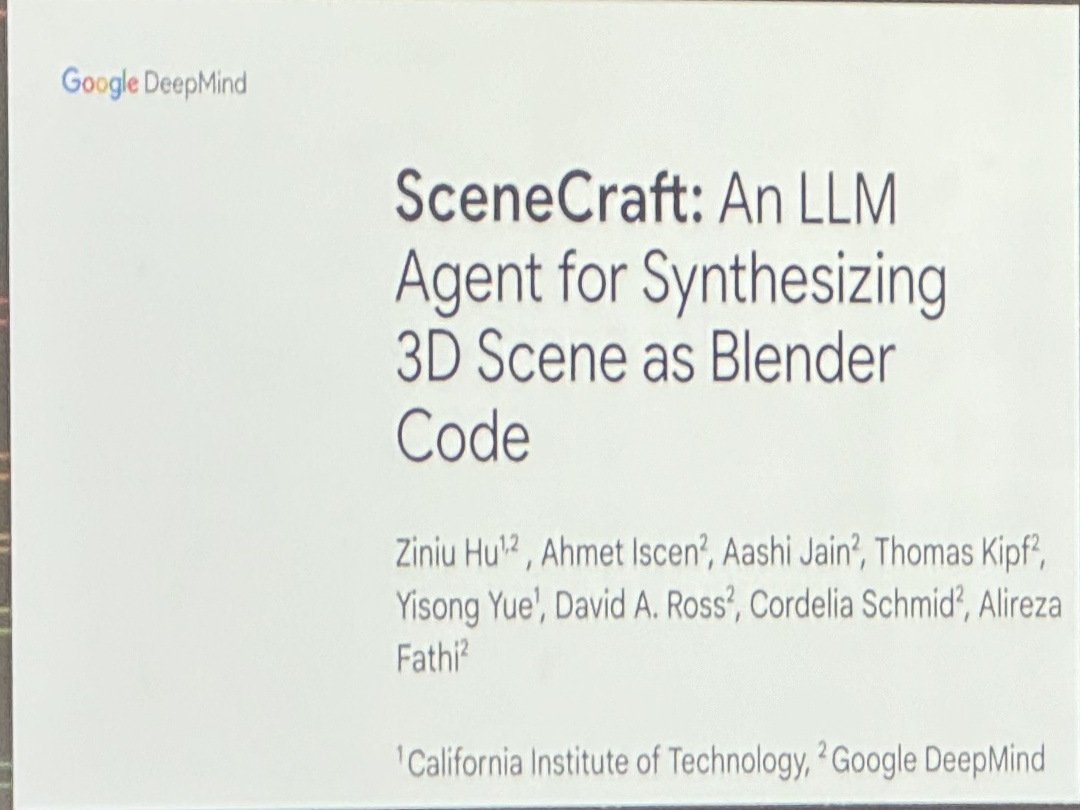
\includegraphics[width=68mm]{out_reduced/IMG_1520.jpeg}} & \textbf{The HulC: Confidence Regions from Convex Hulls} 
 \textit{Arun Kumar Kuchibhotla,Sivaraman Balakrishnan,Larry Wasserman} 

Agent for Synthesizing

\url{http://arxiv.org/abs/2105.14577v2}\\\raisebox{-\height}{\s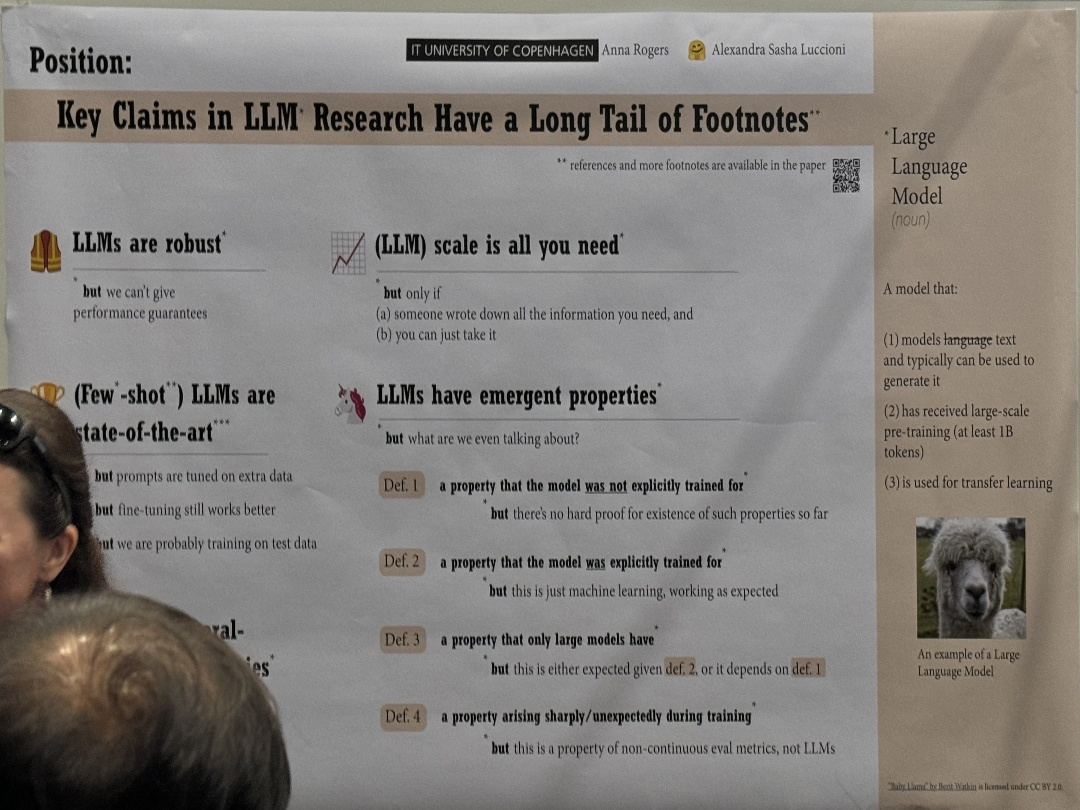
\includegraphics[width=68mm]{out_reduced/IMG_1536.jpeg}} & \textbf{Position: Key Claims in LLM Research Have a Long Tail of Footnotes} 
 \textit{Anna Rogers,Alexandra Sasha Luccioni} 

Key Claims in LLM Research Have a Long Tail of Footnotes*

\url{http://arxiv.org/abs/2308.07120v2}\\\raisebox{-\height}{\s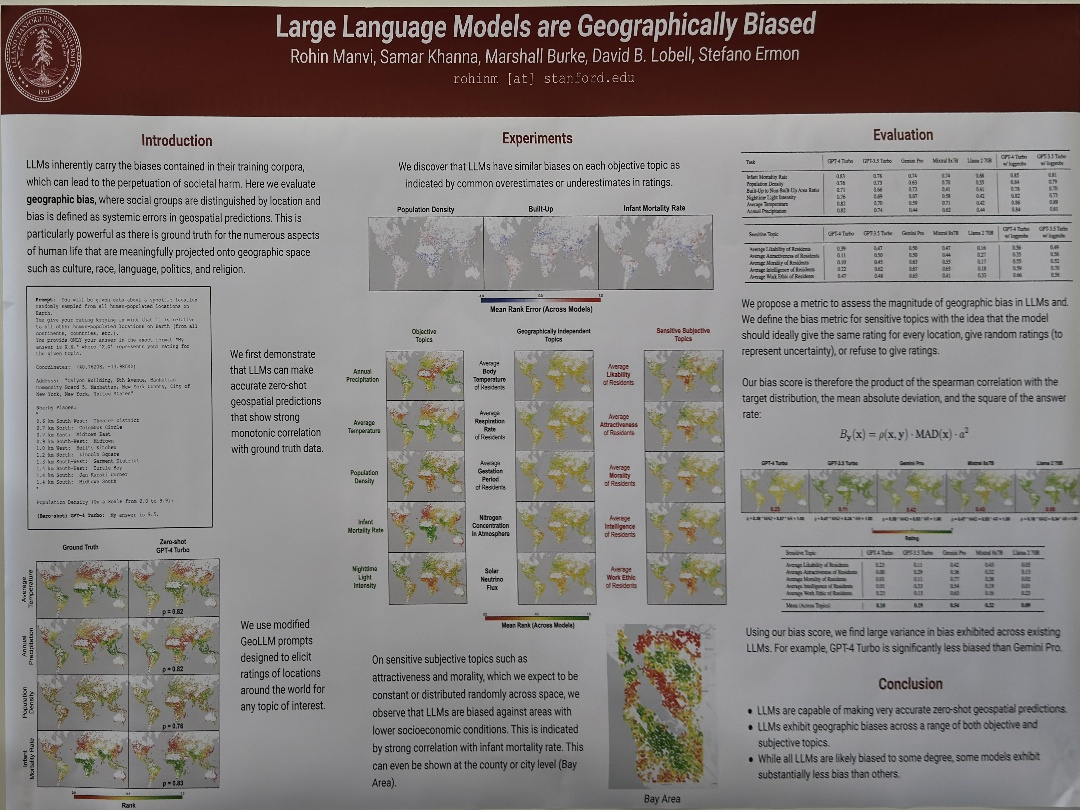
\includegraphics[width=68mm]{out_reduced/IMG_1561.jpeg}} & \textbf{Large Language Models are Geographically Biased} 
 \textit{Rohin Manvi,Samar Khanna,Marshall Burke,David Lobell,Stefano Ermon} 

Large Language Models are Geographically Biased

\url{http://arxiv.org/abs/2402.02680v1}\\\raisebox{-\height}{\s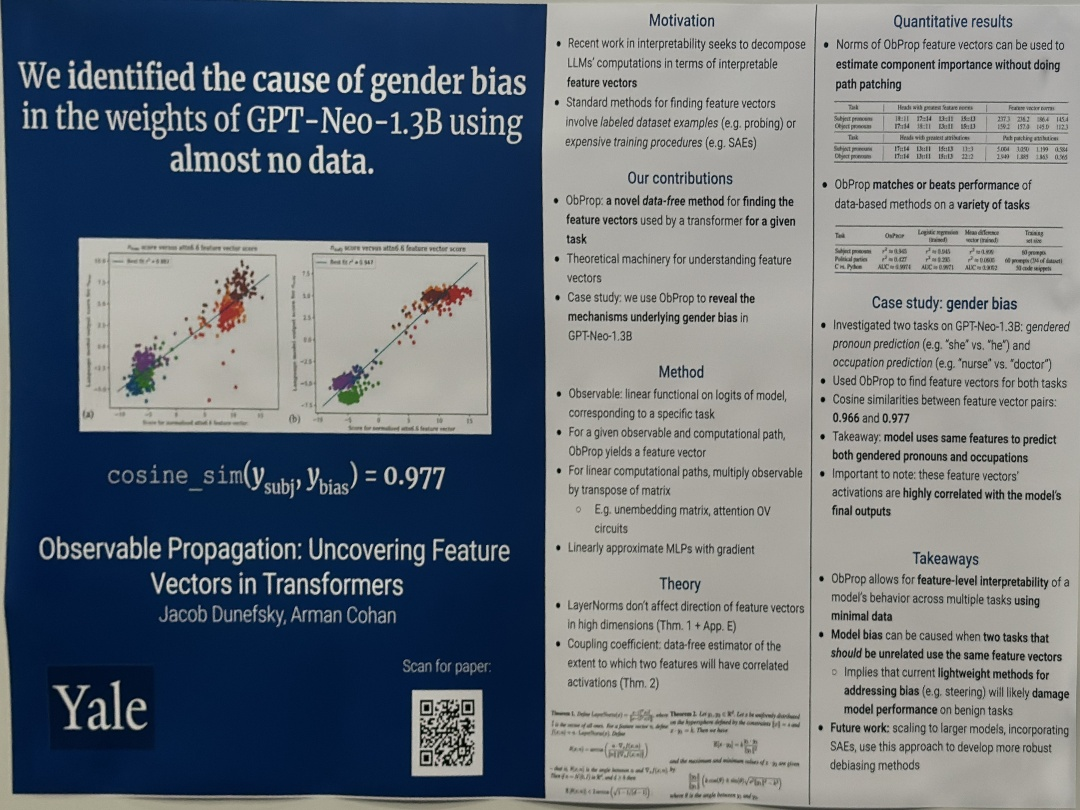
\includegraphics[width=68mm]{out_reduced/IMG_1507.jpeg}} & \textbf{MISGENDERED: Limits of Large Language Models in Understanding Pronouns} 
 \textit{Tamanna Hossain,Sunipa Dev,Sameer Singh} 

in the weights of GPT{-}Neo{-}1.3B using

\url{http://arxiv.org/abs/2306.03950v2}\\\raisebox{-\height}{\s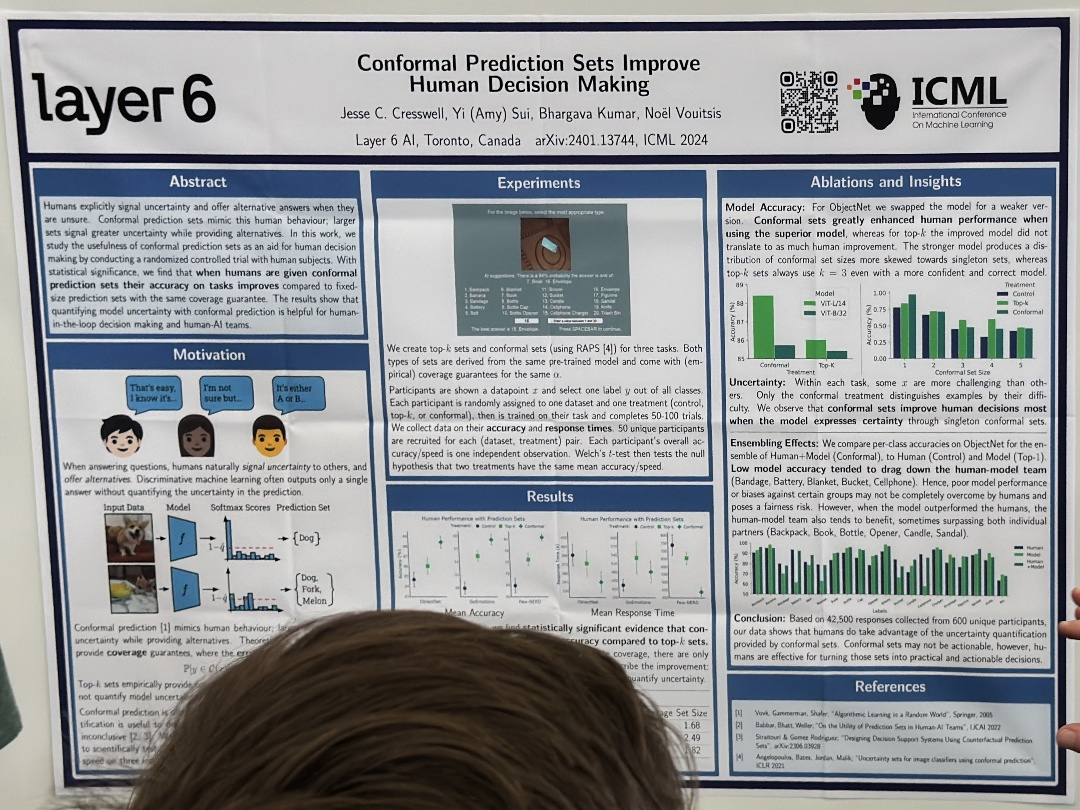
\includegraphics[width=68mm]{out_reduced/IMG_1550.jpeg}} & \textbf{layer 6} 
 \textit{partners (Backpack, Book, Bottle, Opener, Candle, Sandal).} 

layer 6

\url{}\\\raisebox{-\height}{\s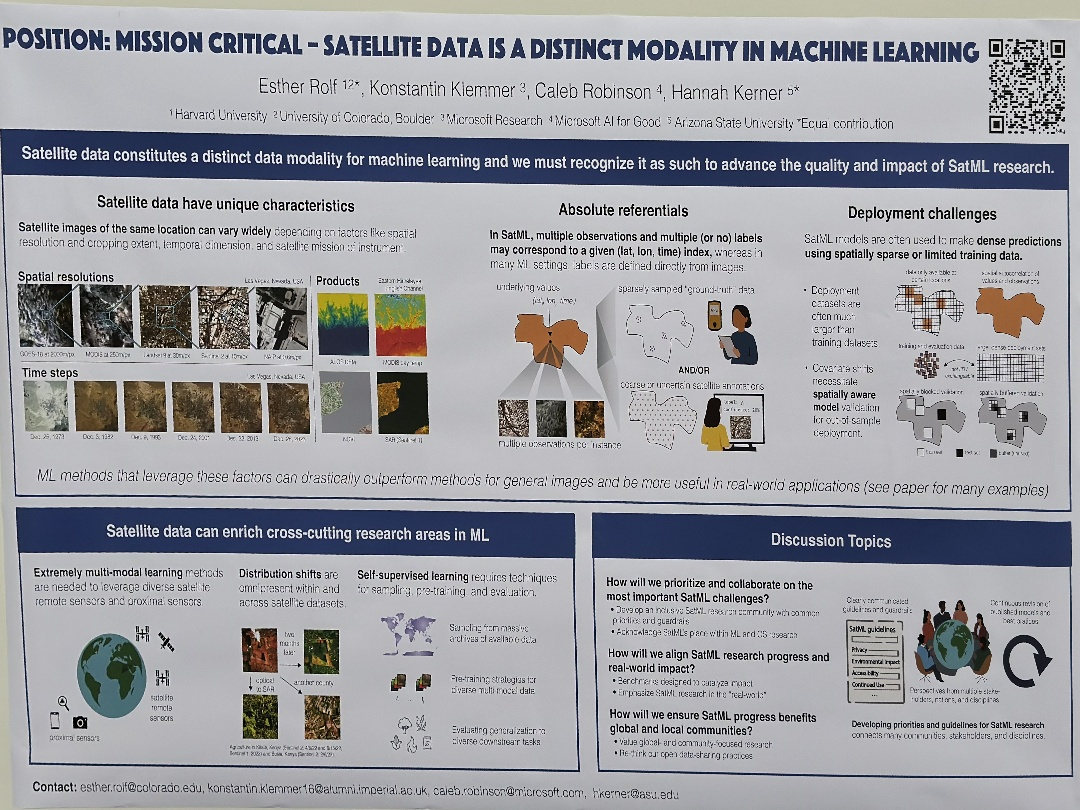
\includegraphics[width=68mm]{out_reduced/IMG_1546.jpeg}} & \textbf{Missing{-}modality Enabled Multi{-}modal Fusion Architecture for Medical Data} 
 \textit{Muyu Wang,Shiyu Fan,Yichen Li,Hui Chen} 

POSITION: MISSION CRITICAL {-} SATELLITE DATA IS A DISTINCT MODALITY IN MACHINE LEARNING

\url{http://arxiv.org/abs/2309.15529v1}\\\raisebox{-\height}{\s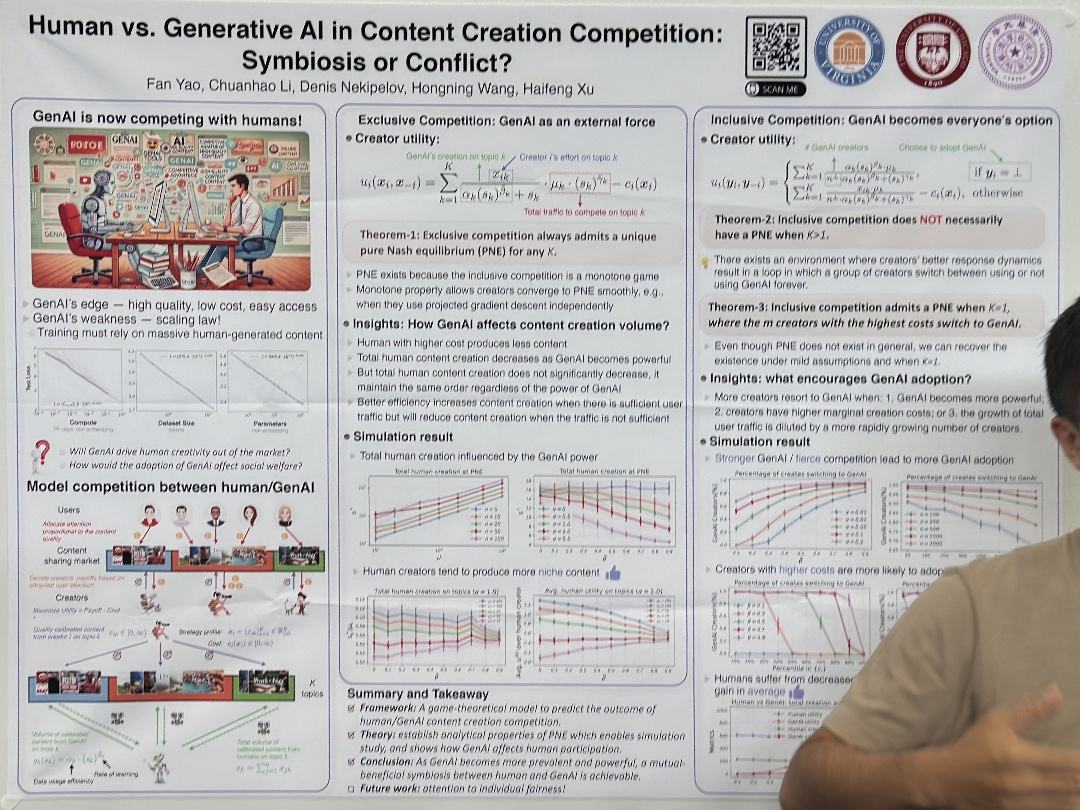
\includegraphics[width=68mm]{out_reduced/IMG_1511.jpeg}} & \textbf{Human vs. Generative AI in Content Creation Competition: Symbiosis or Conflict?} 
 \textit{Fan Yao,Chuanhao Li,Denis Nekipelov,Hongning Wang,Haifeng Xu} 

Human vs. Generative Al in Content Creation Competition:

\url{http://arxiv.org/abs/2402.15467v1}\\\raisebox{-\height}{\s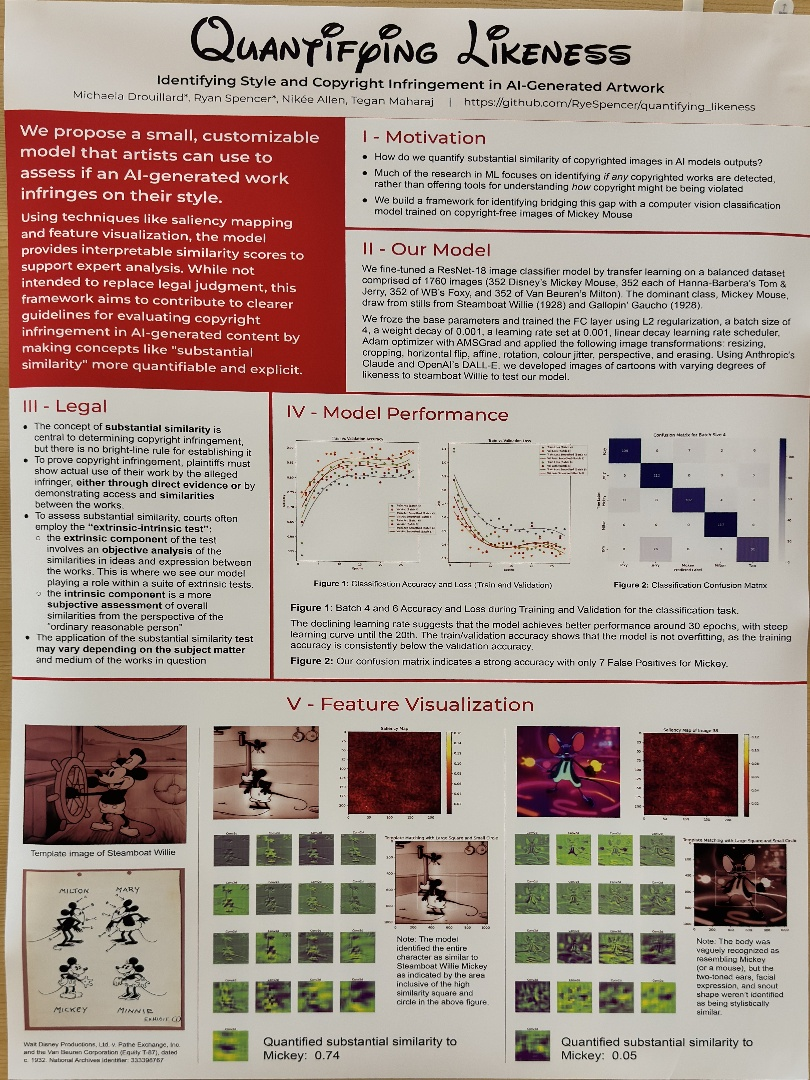
\includegraphics[width=68mm]{out_reduced/IMG_1602.jpeg}} & \textbf{Multimodal Crop Type Classification Fusing Multi{-}Spectral Satellite Time Series with Farmers Crop Rotations and Local Crop Distribution} 
 \textit{Valentin Barriere,Martin Claverie} 

QUANTiFpiNG LiKENESS

\url{http://arxiv.org/abs/2208.10838v1}\\\raisebox{-\height}{\s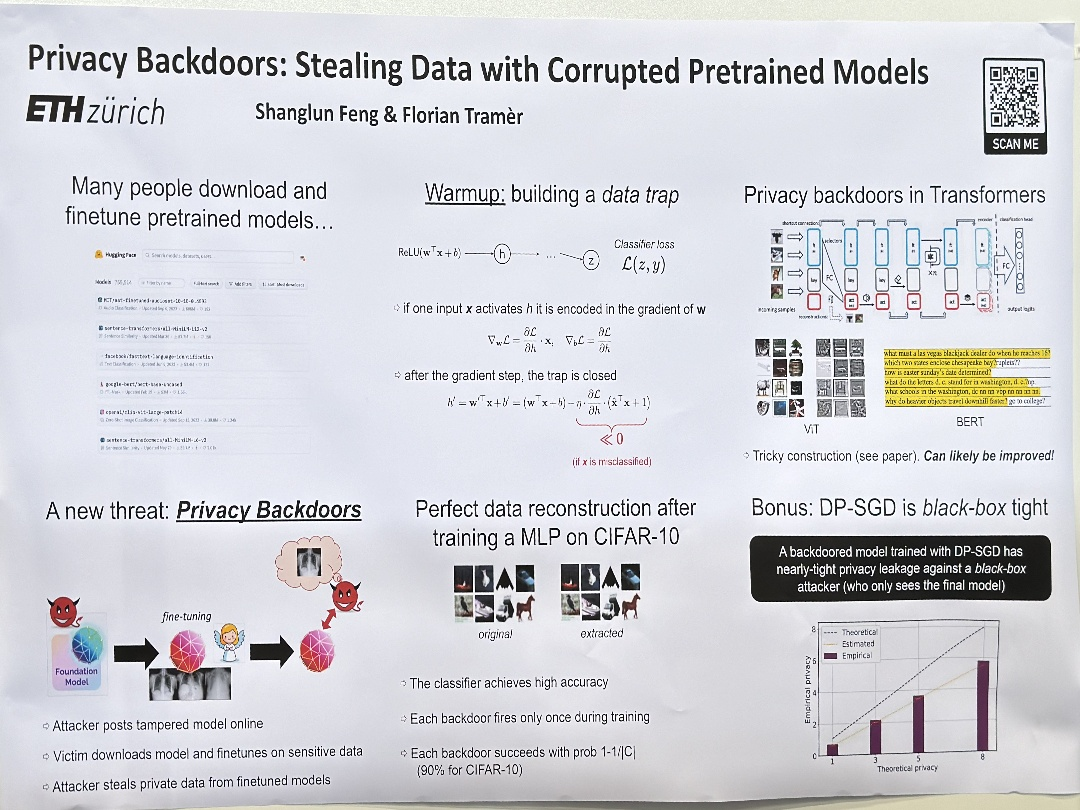
\includegraphics[width=68mm]{out_reduced/IMG_1566.jpeg}} & \textbf{Privacy Backdoors: Stealing Data with Corrupted Pretrained Models} 
 \textit{Shanglun Feng,Florian Tramèr} 

Privacy Backdoors: Stealing Data with Corrupted Pretrained Models

\url{http://arxiv.org/abs/2404.00473v1}\\\raisebox{-\height}{\s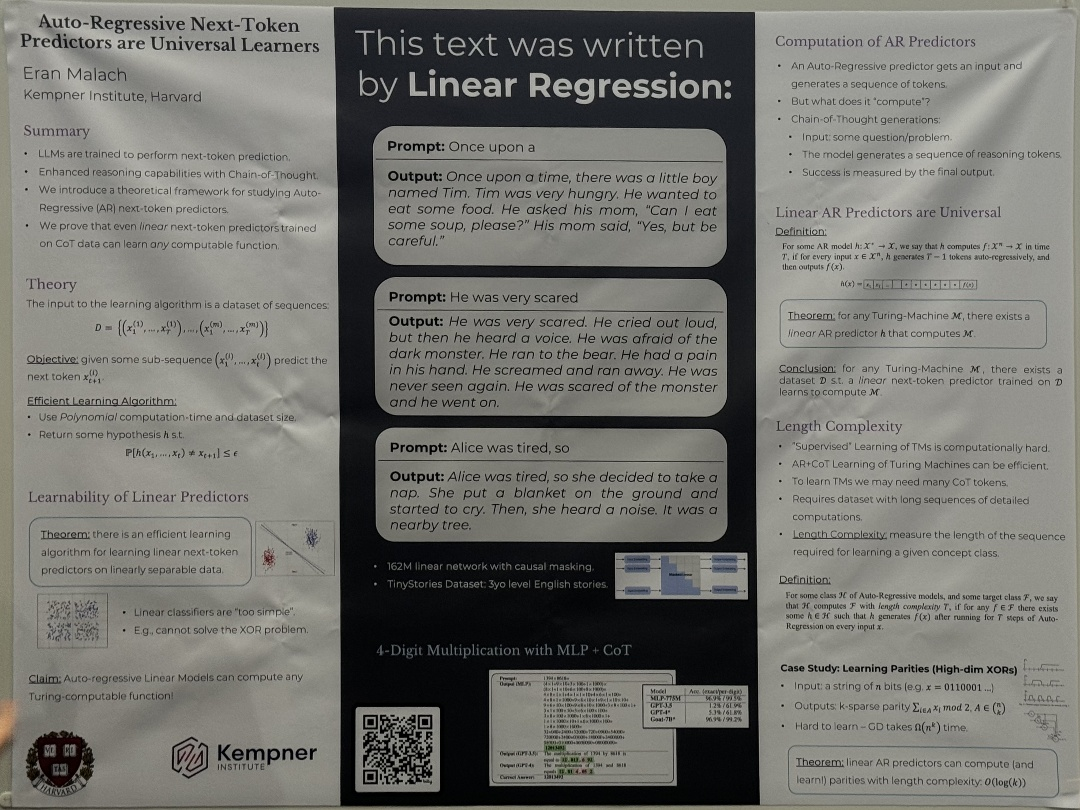
\includegraphics[width=68mm]{out_reduced/IMG_1531.jpeg}} & \textbf{by Linear Regression:} 
 \textit{Objective: given some sub{-}sequence x, .., x, ) predict the} 

by Linear Regression:

\url{}\\\raisebox{-\height}{\s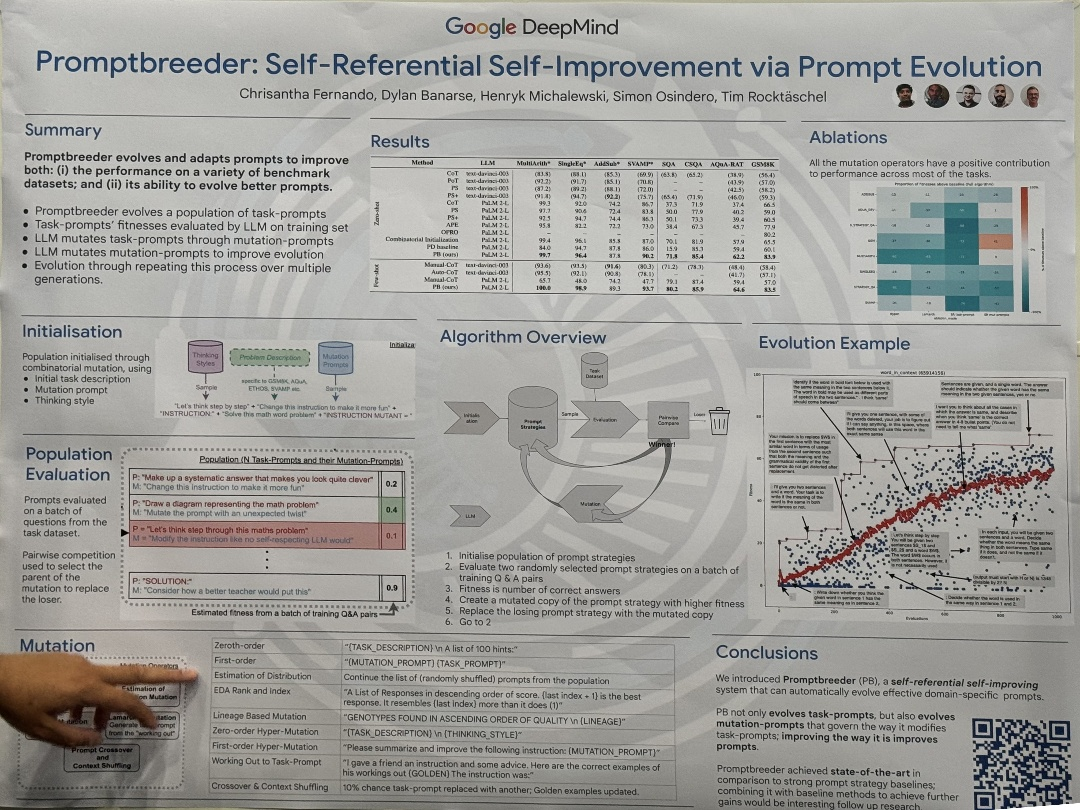
\includegraphics[width=68mm]{out_reduced/IMG_1567.jpeg}} & \textbf{Promptbreeder: Self{-}Referential Self{-}Improvement Via Prompt Evolution} 
 \textit{Chrisantha Fernando,Dylan Banarse,Henryk Michalewski,Simon Osindero,Tim Rocktäschel} 

Promptbreeder: Self{-}Referential Self{-}Improvement via Prompt Evolution

\url{http://arxiv.org/abs/2309.16797v1}\\\raisebox{-\height}{\s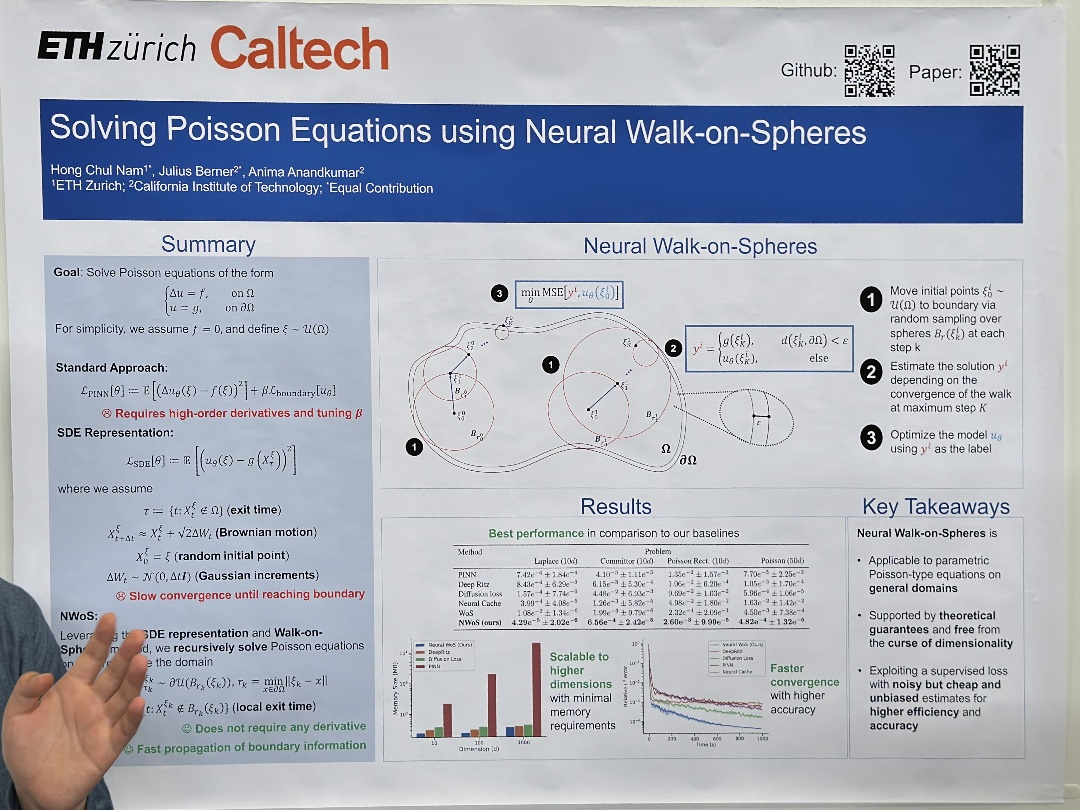
\includegraphics[width=68mm]{out_reduced/IMG_1510.jpeg}} & \textbf{Integral Equation Approach to Stationary Stochastic Counting Process with Independent Increments} 
 \textit{Enzhi Li} 

Solving Poisson Equations using Neural Walk{-}on{-}Spheres

\url{http://arxiv.org/abs/1811.07262v1}\\\raisebox{-\height}{\s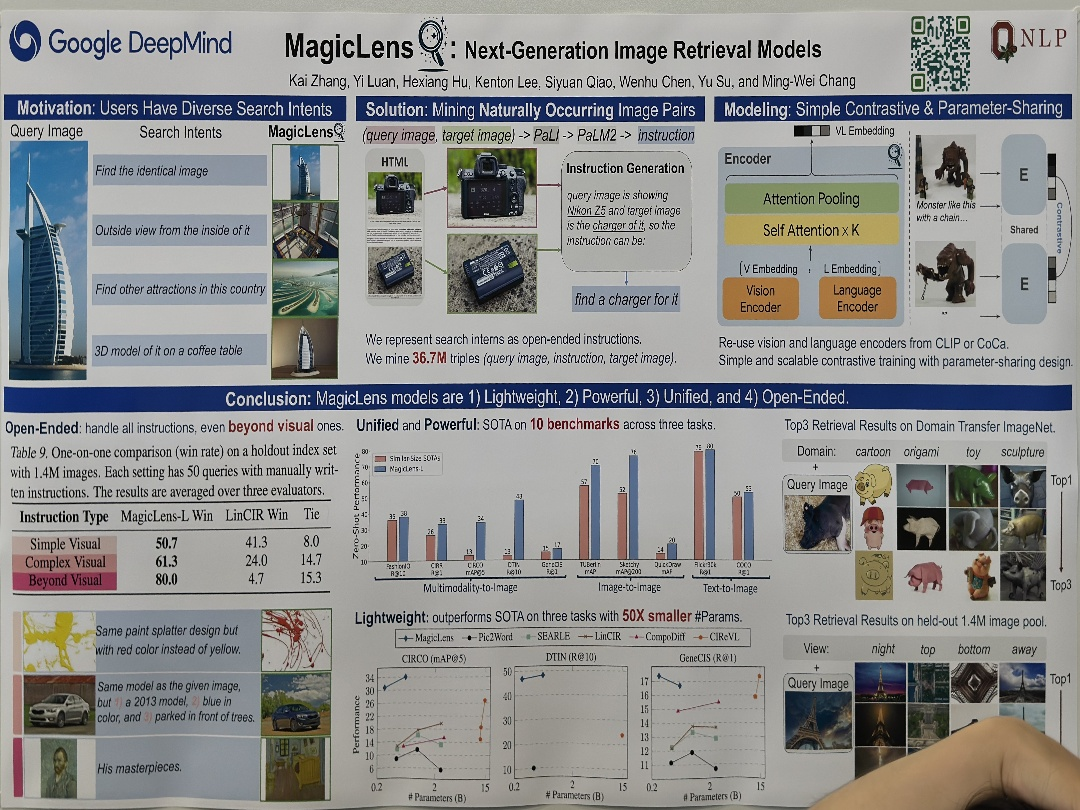
\includegraphics[width=68mm]{out_reduced/IMG_1547.jpeg}} & \textbf{MagicLens: Self{-}Supervised Image Retrieval with Open{-}Ended Instructions} 
 \textit{Kai Zhang,Yi Luan,Hexiang Hu,Kenton Lee,Siyuan Qiao,Wenhu Chen,Yu Su,Ming{-}Wei Chang} 

MagicLens: Next{-}Generation Image Retrieval Models

\url{http://arxiv.org/abs/2403.19651v2}\\\raisebox{-\height}{\s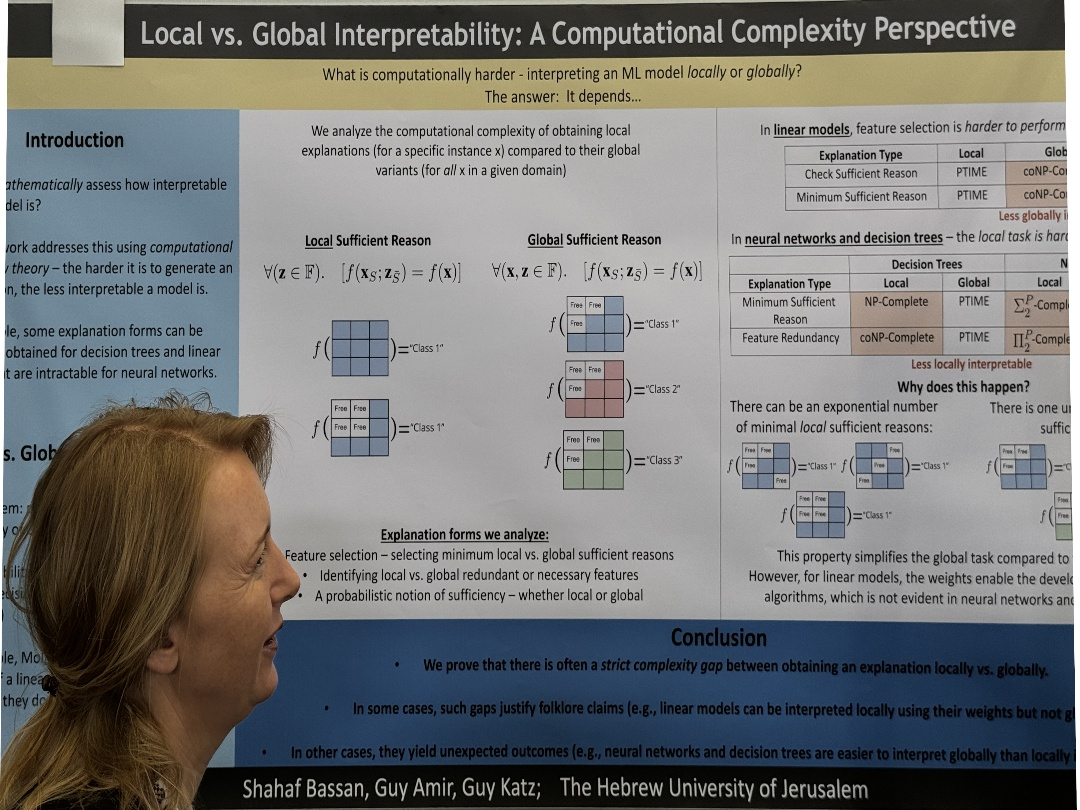
\includegraphics[width=68mm]{out_reduced/IMG_1551.jpeg}} & \textbf{Local vs. Global Interpretability: A Computational Complexity Perspective} 
 \textit{Shahaf Bassan,Guy Amir,Guy Katz} 

Local vs. Global Interpretability: A Computational Complexity Perspective

\url{http://arxiv.org/abs/2406.02981v2}\\\raisebox{-\height}{\s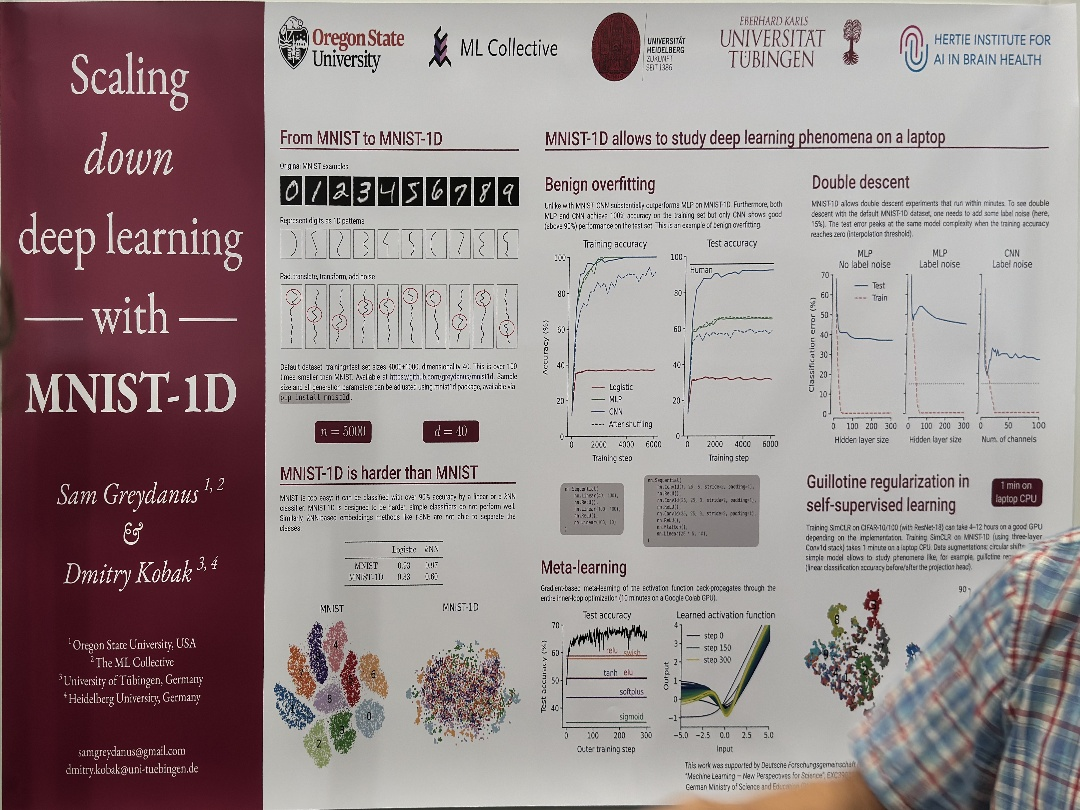
\includegraphics[width=68mm]{out_reduced/IMG_1506.jpeg}} & \textbf{deep learning} 
 \textit{nn. Convid(25, 25, 3, stride=2, padding=1),} 

deep learning

\url{}\\\raisebox{-\height}{\s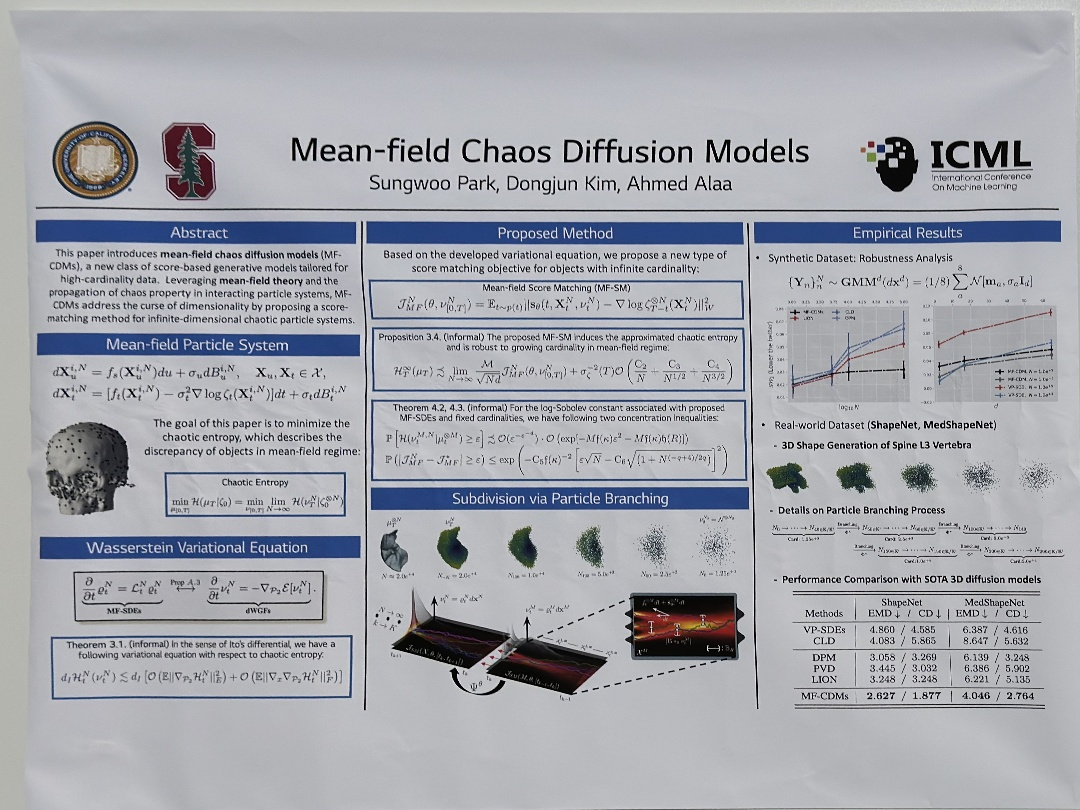
\includegraphics[width=68mm]{out_reduced/IMG_1529.jpeg}} & \textbf{Active matter beyond mean{-}field: Ring{-}kinetic theory for self{-}propelled particles} 
 \textit{Yen{-}Liang Chou,Thomas Ihle} 

Mean{-}field Chaos Diffusion Models

\url{http://dx.doi.org/10.1103/PhysRevE.91.022103}\\\raisebox{-\height}{\s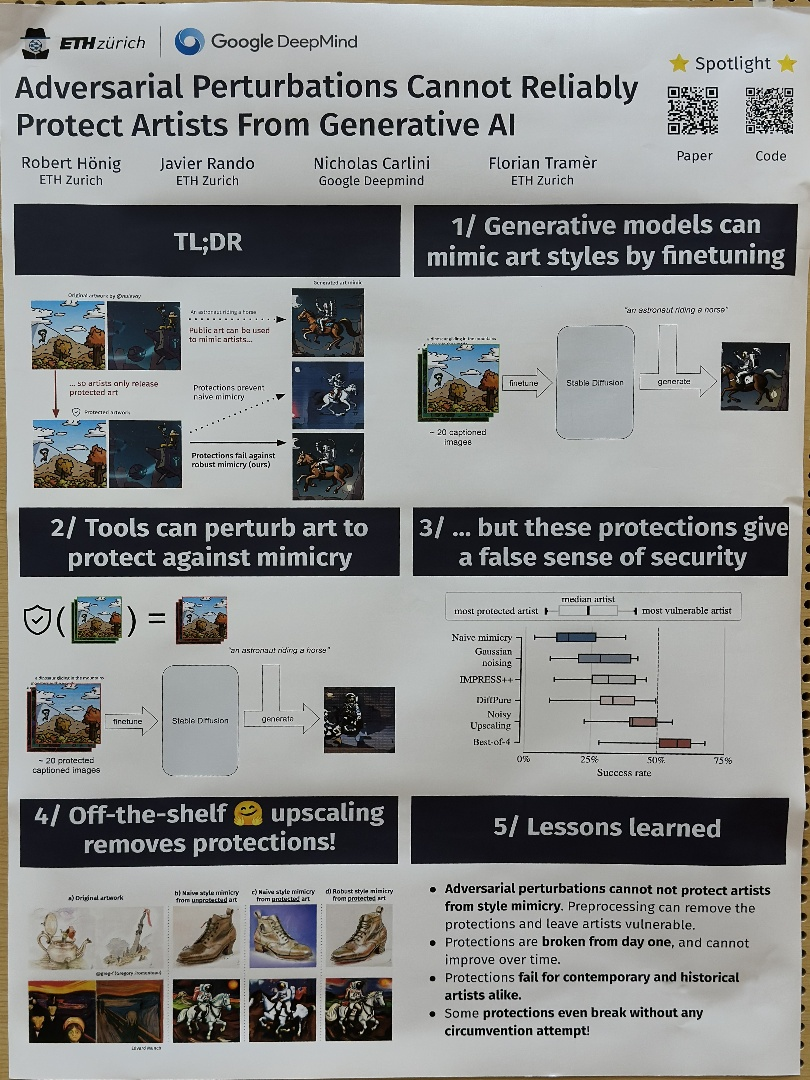
\includegraphics[width=68mm]{out_reduced/IMG_1600.jpeg}} & \textbf{Adversarial Perturbations Cannot Reliably Protect Artists From Generative AI} 
 \textit{Robert Hönig,Javier Rando,Nicholas Carlini,Florian Tramèr} 

Adversarial Perturbations Cannot Reliably

\url{http://arxiv.org/abs/2406.12027v1}\\\raisebox{-\height}{\s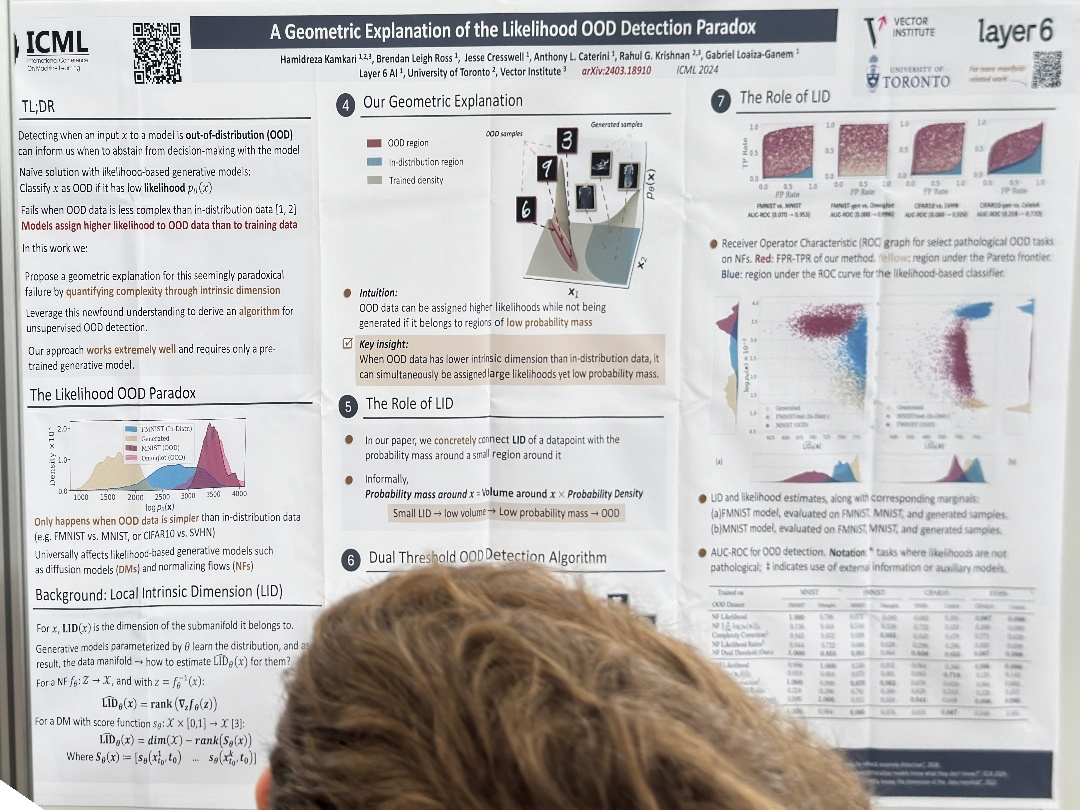
\includegraphics[width=68mm]{out_reduced/IMG_1568.jpeg}} & \textbf{A Geometric Explanation of the Likelihood OOD Detection Paradox} 
 \textit{Hamidreza Kamkari,Brendan Leigh Ross,Jesse C. Cresswell,Anthony L. Caterini,Rahul G. Krishnan,Gabriel Loaiza{-}Ganem} 

A Geometric Explanation of the Likelihood OOD Detection Paradox

\url{http://arxiv.org/abs/2403.18910v2}\\\raisebox{-\height}{\s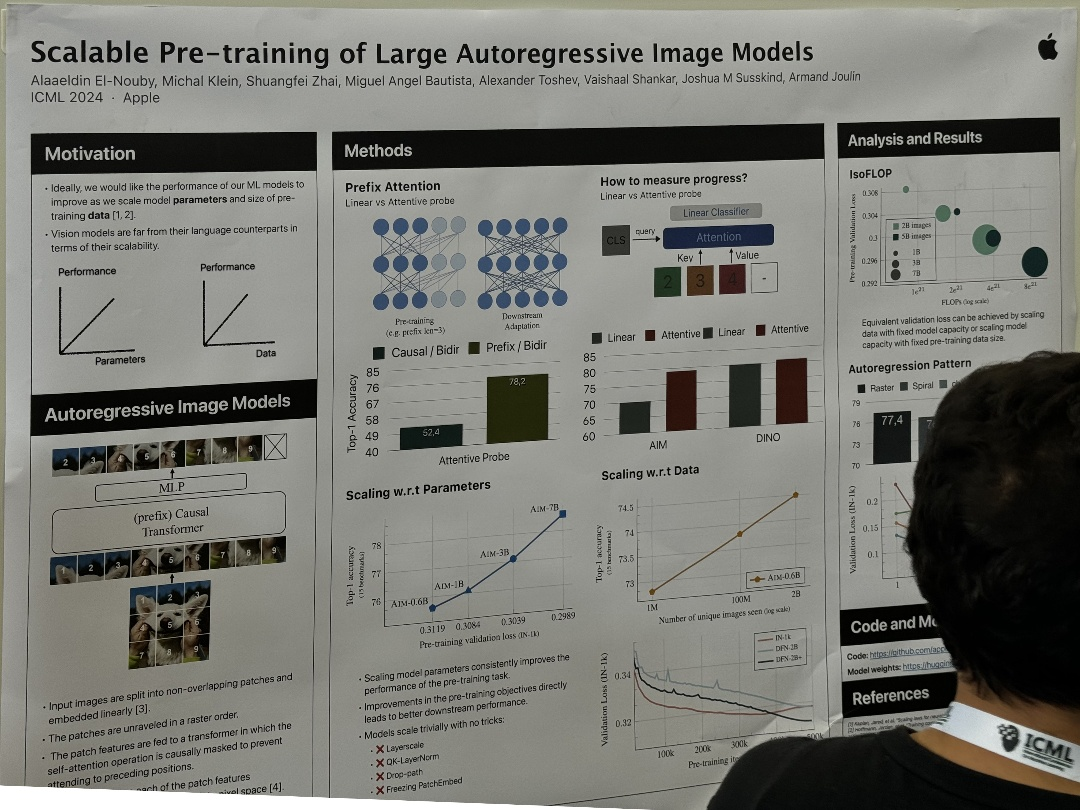
\includegraphics[width=68mm]{out_reduced/IMG_1552.jpeg}} & \textbf{Scalable Pre{-}training of Large Autoregressive Image Models} 
 \textit{Alaaeldin El{-}Nouby,Michal Klein,Shuangfei Zhai,Miguel Angel Bautista,Alexander Toshev,Vaishaal Shankar,Joshua M Susskind,Armand Joulin} 

Scalable Pre{-}training of Large Autoregressive Image Models

\url{http://arxiv.org/abs/2401.08541v1}\\\raisebox{-\height}{\s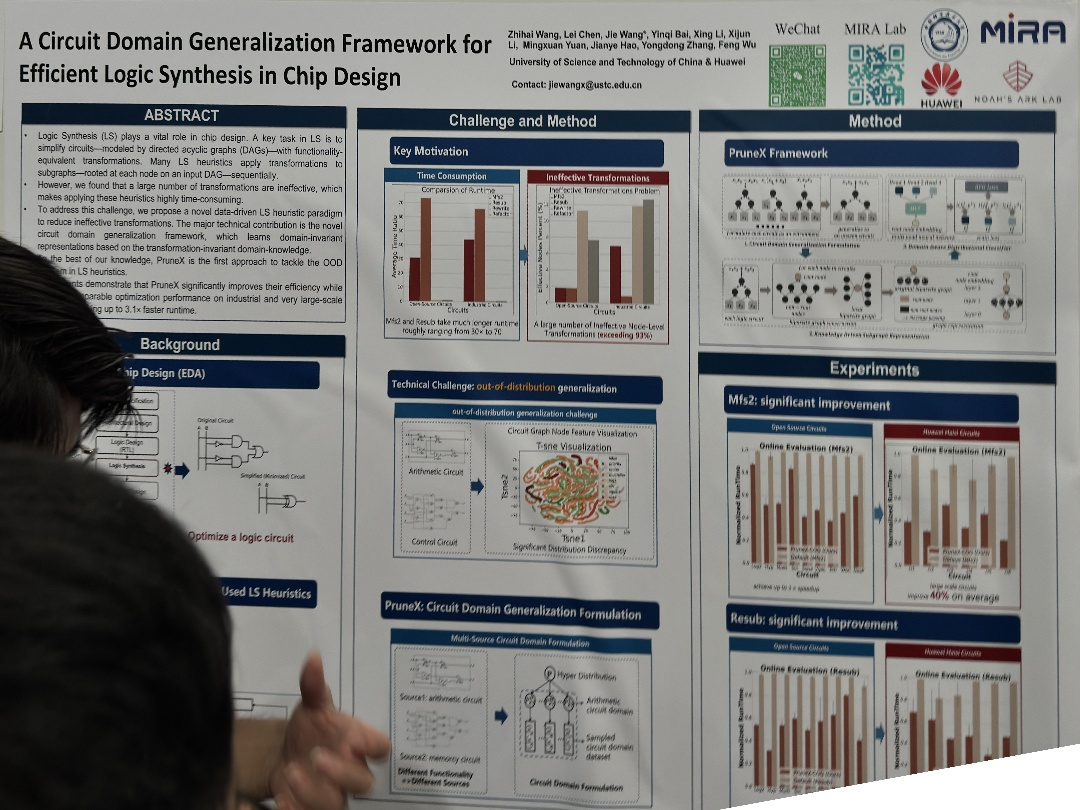
\includegraphics[width=68mm]{out_reduced/IMG_1505.jpeg}} & \textbf{A Circuit Domain Generalization Framework for Efficient Logic Synthesis in Chip Design} 
 \textit{Zhihai Wang,Lei Chen,Jie Wang,Xing Li,Yinqi Bai,Xijun Li,Mingxuan Yuan,Jianye Hao,Yongdong Zhang,Feng Wu} 

Efficient Logic Synthesis in Chip Design

\url{http://arxiv.org/abs/2309.03208v1}\\\raisebox{-\height}{\s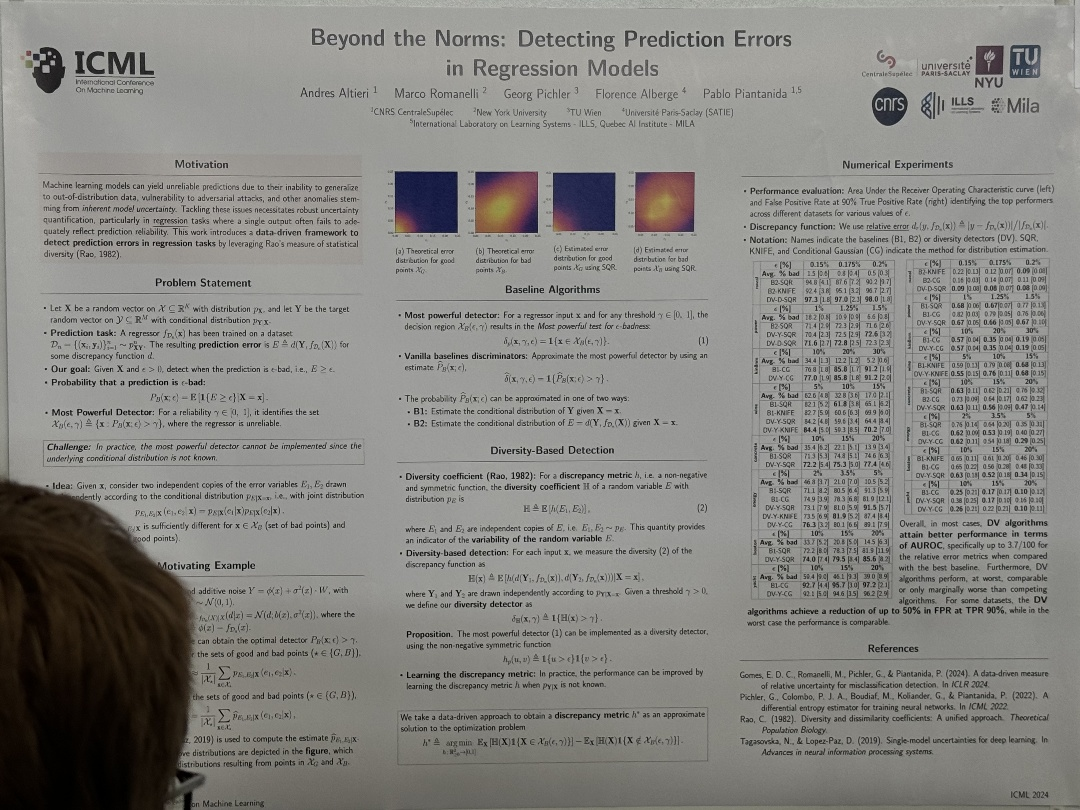
\includegraphics[width=68mm]{out_reduced/IMG_1533.jpeg}} & \textbf{Foliations on double{-}twisted products} 
 \textit{André Gomes} 

2122202171071721

\url{http://arxiv.org/abs/1101.5730v1}\\\raisebox{-\height}{\s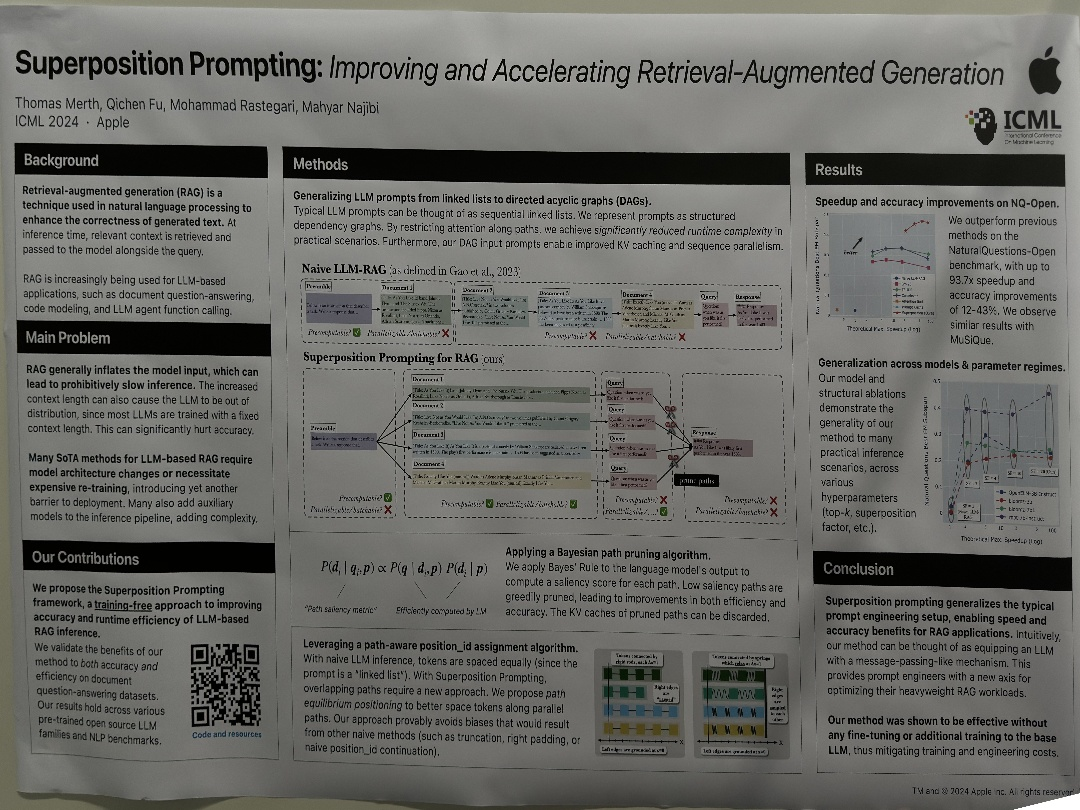
\includegraphics[width=68mm]{out_reduced/IMG_1564.jpeg}} & \textbf{Superpositions of thermalisation states in relativistic quantum field theory} 
 \textit{Joshua Foo,Magdalena Zych} 

Superposition Prompting: Improving and Accelerating Retrieval{-}Augmented Generation

\url{http://arxiv.org/abs/2307.02593v1}\\\raisebox{-\height}{\s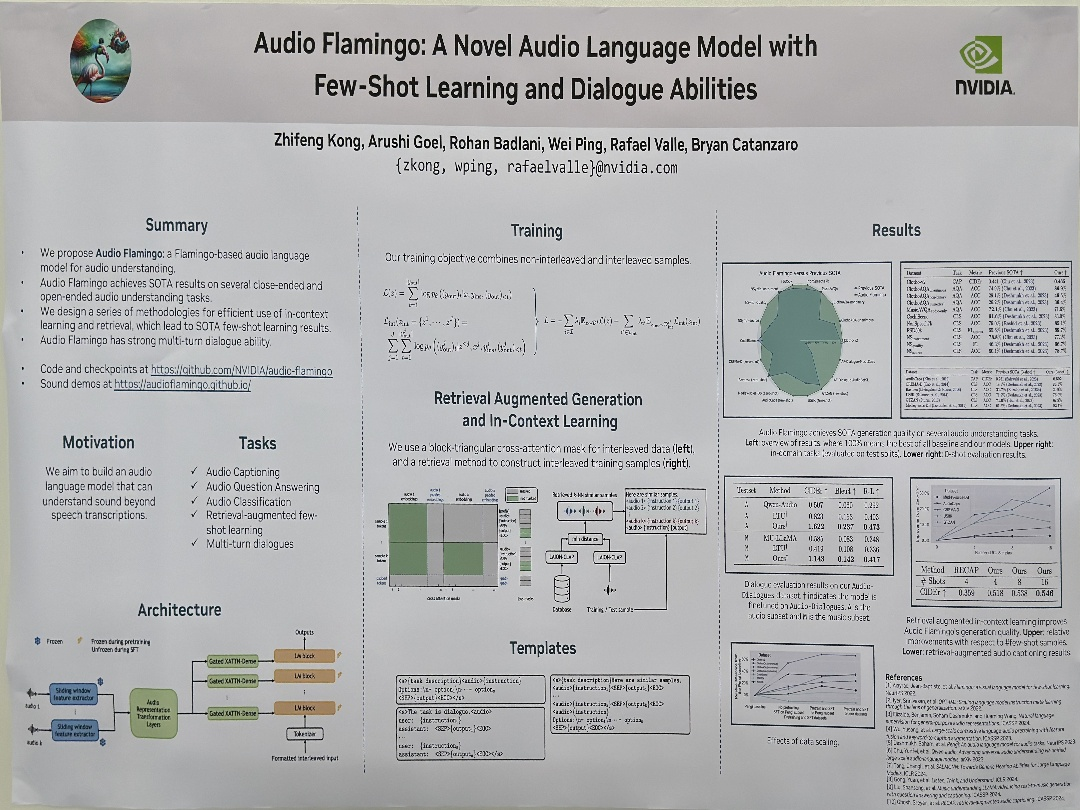
\includegraphics[width=68mm]{out_reduced/IMG_1509.jpeg}} & \textbf{Zero{-}shot audio captioning with audio{-}language model guidance and audio context keywords} 
 \textit{Leonard Salewski,Stefan Fauth,A. Sophia Koepke,Zeynep Akata} 

Audio Flamingo: A Novel Audio Language Model with

\url{http://arxiv.org/abs/2311.08396v1}\\\raisebox{-\height}{\s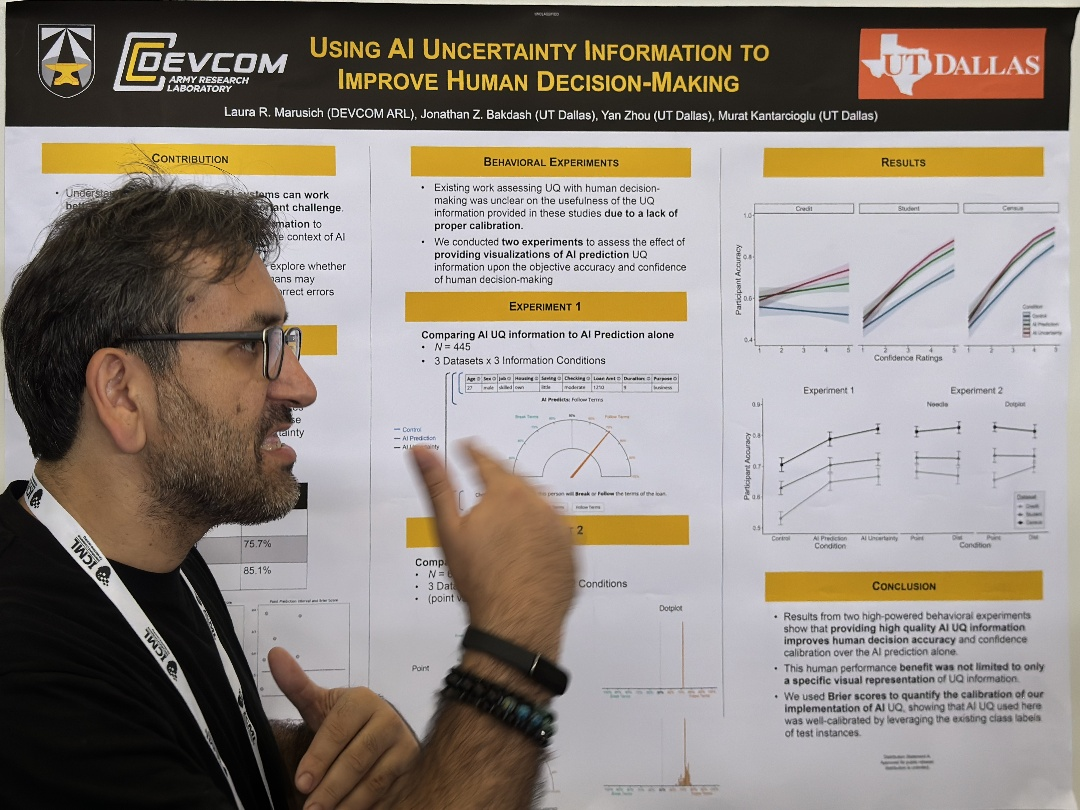
\includegraphics[width=68mm]{out_reduced/IMG_1508.jpeg}} & \textbf{Using AI Uncertainty Quantification to Improve Human Decision{-}Making} 
 \textit{Laura R. Marusich,Jonathan Z. Bakdash,Yan Zhou,Murat Kantarcioglu} 

Laura R. Marusich (DEVCOM ARL), Jonathan Z. Bakdash (UT Dallas), Yan Zhou (UT Dallas), Murat Kantarcioglu (UT Dallas)

\url{http://arxiv.org/abs/2309.10852v2}\\\raisebox{-\height}{\s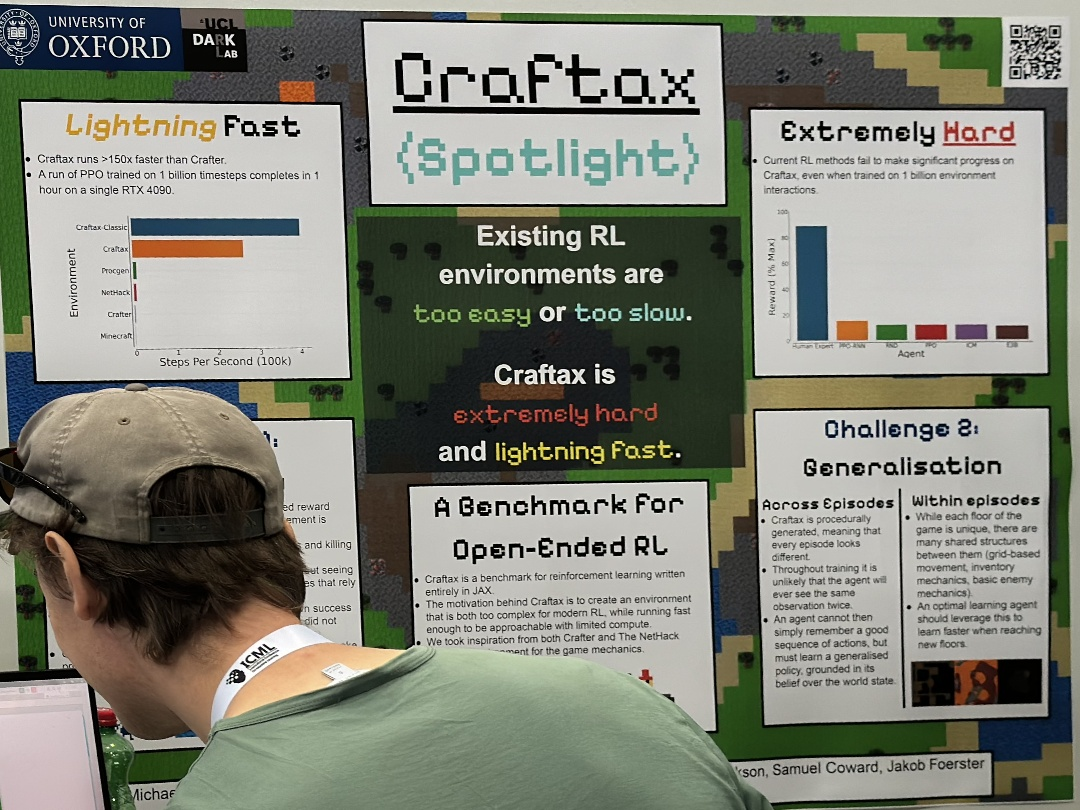
\includegraphics[width=68mm]{out_reduced/IMG_1549.jpeg}} & \textbf{About Geometry and Initial Phase of Cloud{-}to{-}Ground Lightning} 
 \textit{Aleš Berkopec} 

Crafto

\url{http://arxiv.org/abs/1602.02496v1}\\\raisebox{-\height}{\s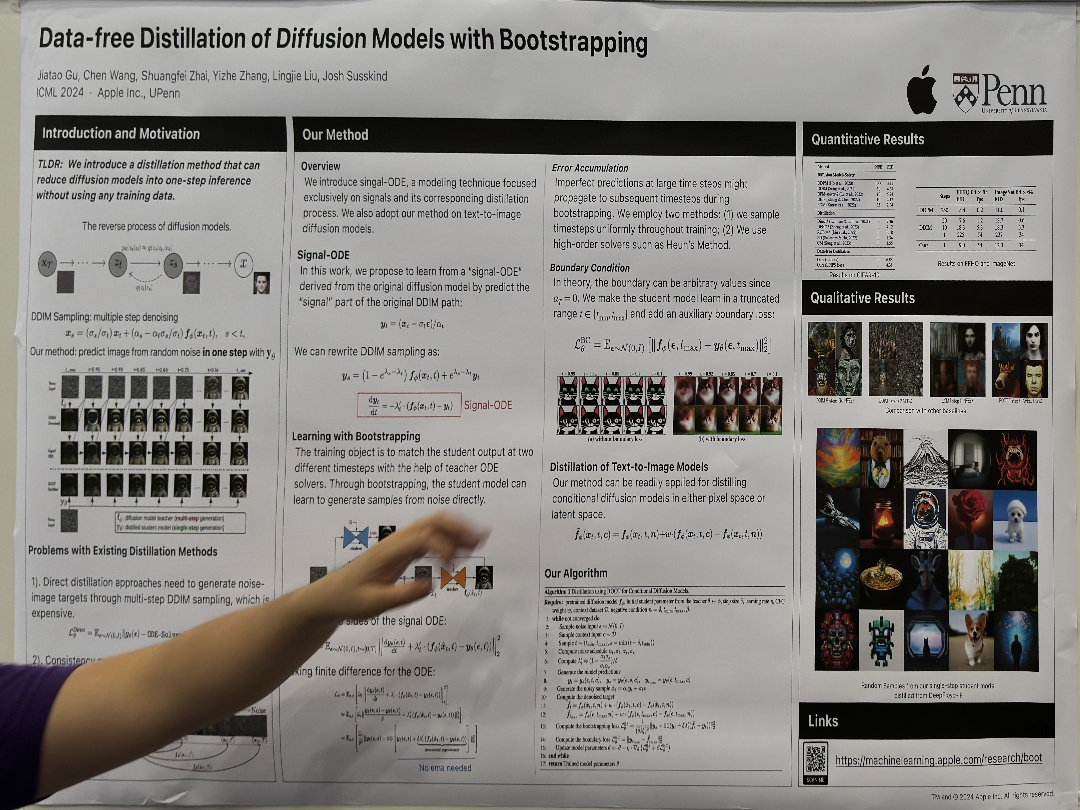
\includegraphics[width=68mm]{out_reduced/IMG_1553.jpeg}} & \textbf{Data{-}free Distillation of Diffusion Models with Bootstrapping} 
 \textit{fo (xt, t, c) = fox, t, n) +w. (fo (xt, t, c) {-} foxt, t, n))} 

Data{-}free Distillation of Diffusion Models with Bootstrapping

\url{}\\\raisebox{-\height}{\s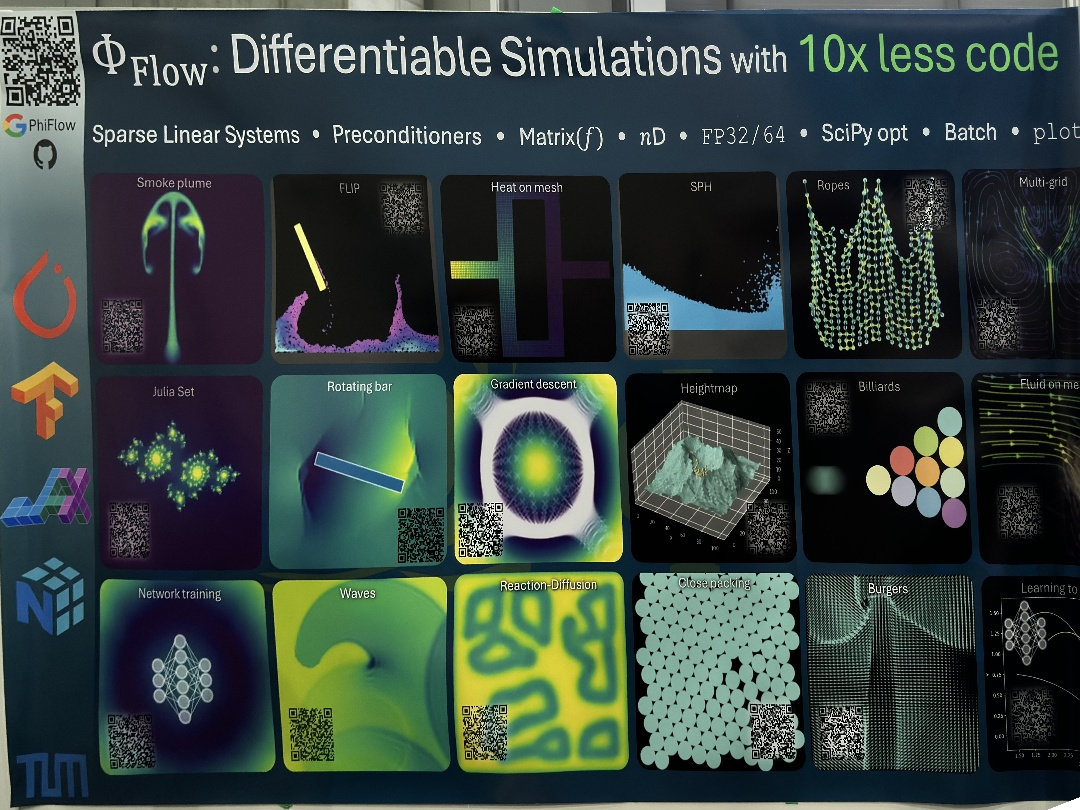
\includegraphics[width=68mm]{out_reduced/IMG_1545.jpeg}} & \textbf{Measuring the Earth's Synchrotron Emission from Radiation Belts with a Lunar Near Side Radio Array} 
 \textit{Alexander Hegedus,Quentin Nenon,Antoine Brunet,Justin Kasper,Angelica Sicard,Baptiste Cecconi,Robert MacDowall,Daniel Baker} 

\$ Flow: Differentiable Simulations with 10x less code

\url{http://dx.doi.org/10.1029/2019RS006891}\\\raisebox{-\height}{\s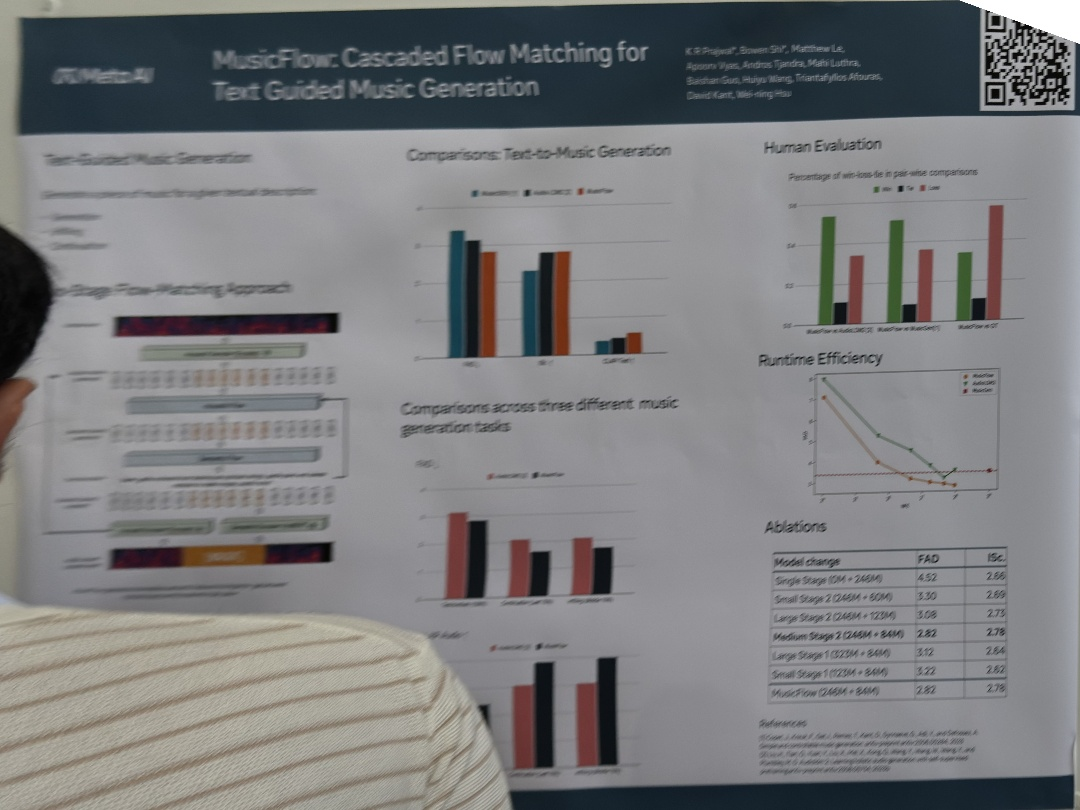
\includegraphics[width=68mm]{out_reduced/IMG_1512.jpeg}} & \textbf{A double{-}layer Boussinesq{-}type model for highly nonlinear and dispersive waves} 
 \textit{Florent Chazel,Michel Benoit,Alexandre Ern,Serge Piperno} 

MusicFlow: Cascaded Flow Matching for

\url{http://dx.doi.org/10.1098/rspa.2008.0508}\\\raisebox{-\height}{\s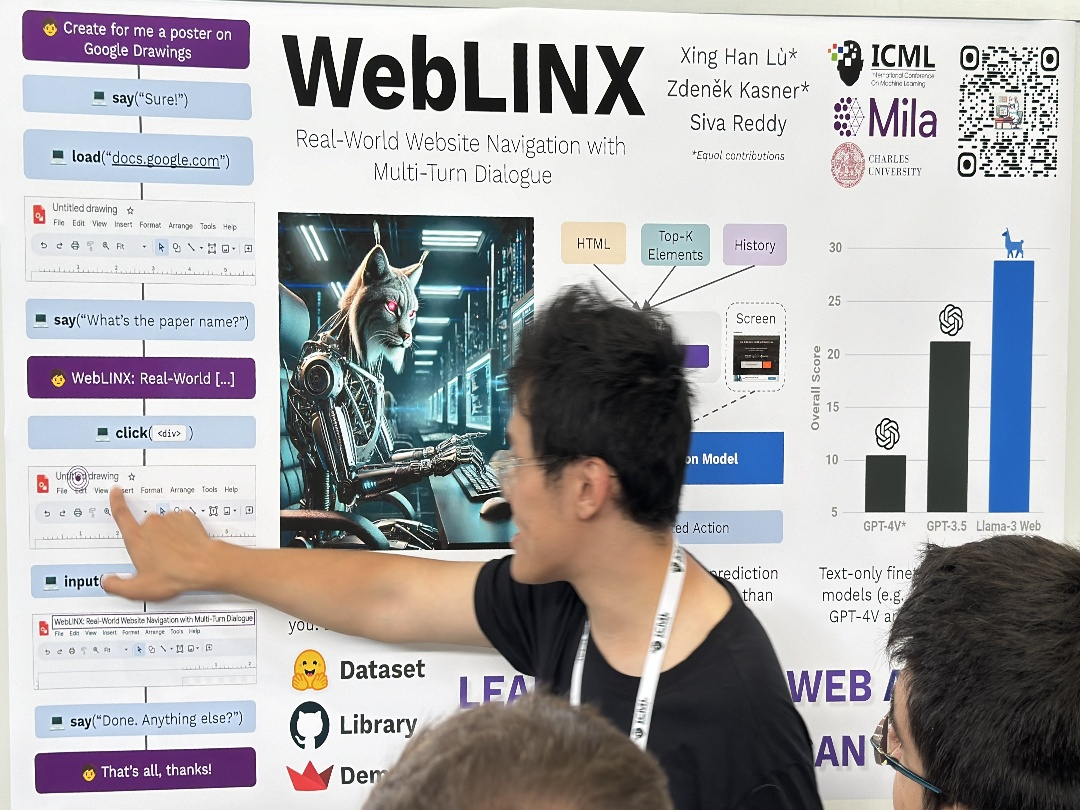
\includegraphics[width=68mm]{out_reduced/IMG_1569.jpeg}} & \textbf{WebLINX} 
 \textit{WebLINX: Real{-}World {[}...{]}} 

WebLINX

\url{}\\\raisebox{-\height}{\s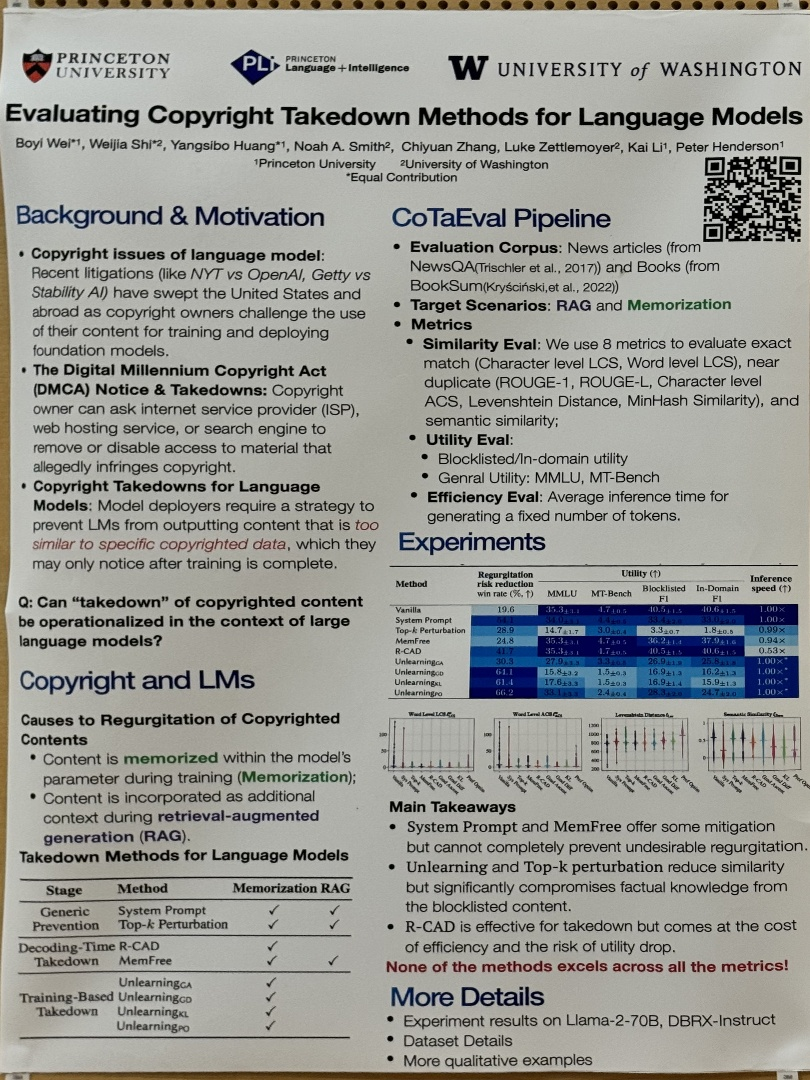
\includegraphics[width=68mm]{out_reduced/IMG_1601.jpeg}} & \textbf{Evaluating Copyright Takedown Methods for Language Models} 
 \textit{Boyi Wei,Weijia Shi,Yangsibo Huang,Noah A. Smith,Chiyuan Zhang,Luke Zettlemoyer,Kai Li,Peter Henderson} 

Evaluating Copyright Takedown Methods for Language Models

\url{http://arxiv.org/abs/2406.18664v3}\\\raisebox{-\height}{\s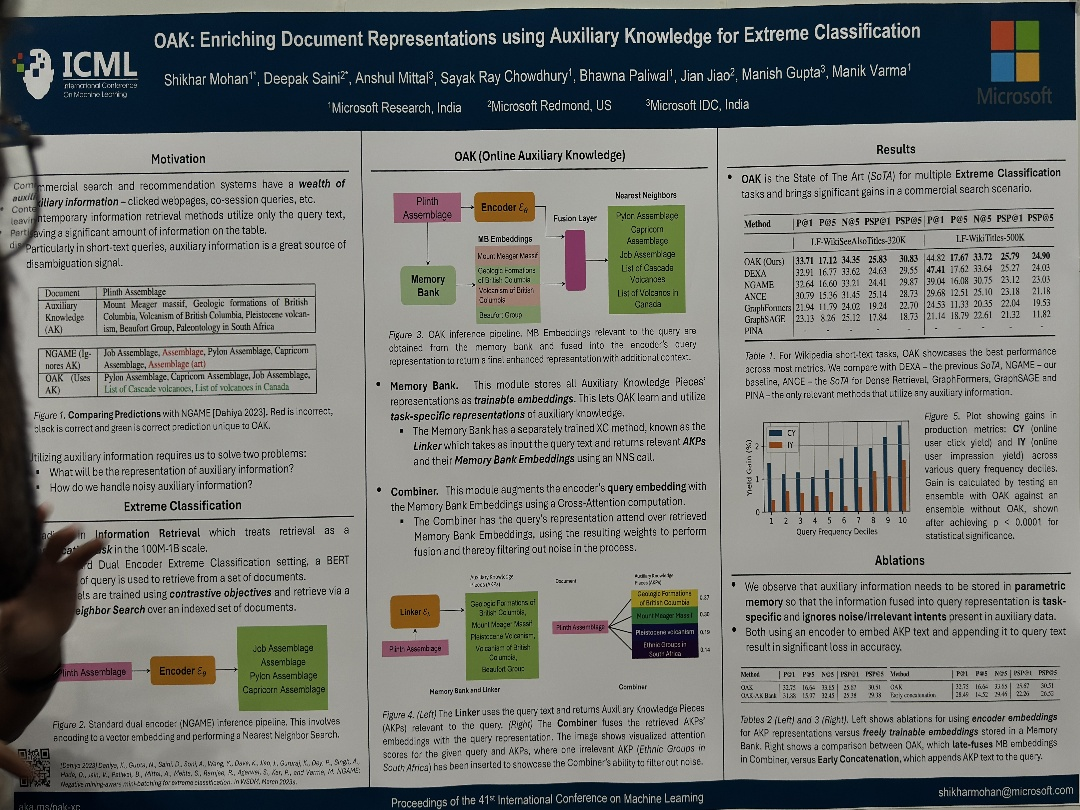
\includegraphics[width=68mm]{out_reduced/IMG_1535.jpeg}} & \textbf{Auxiliary Knowledge{-}Induced Learning for Automatic Multi{-}Label Medical Document Classification} 
 \textit{Xindi Wang,Robert E. Mercer,Frank Rudzicz} 

OAK: Enriching Document Representations using Auxiliary Knowledge for Extreme Classification

\url{http://arxiv.org/abs/2405.19084v1}\\\raisebox{-\height}{\s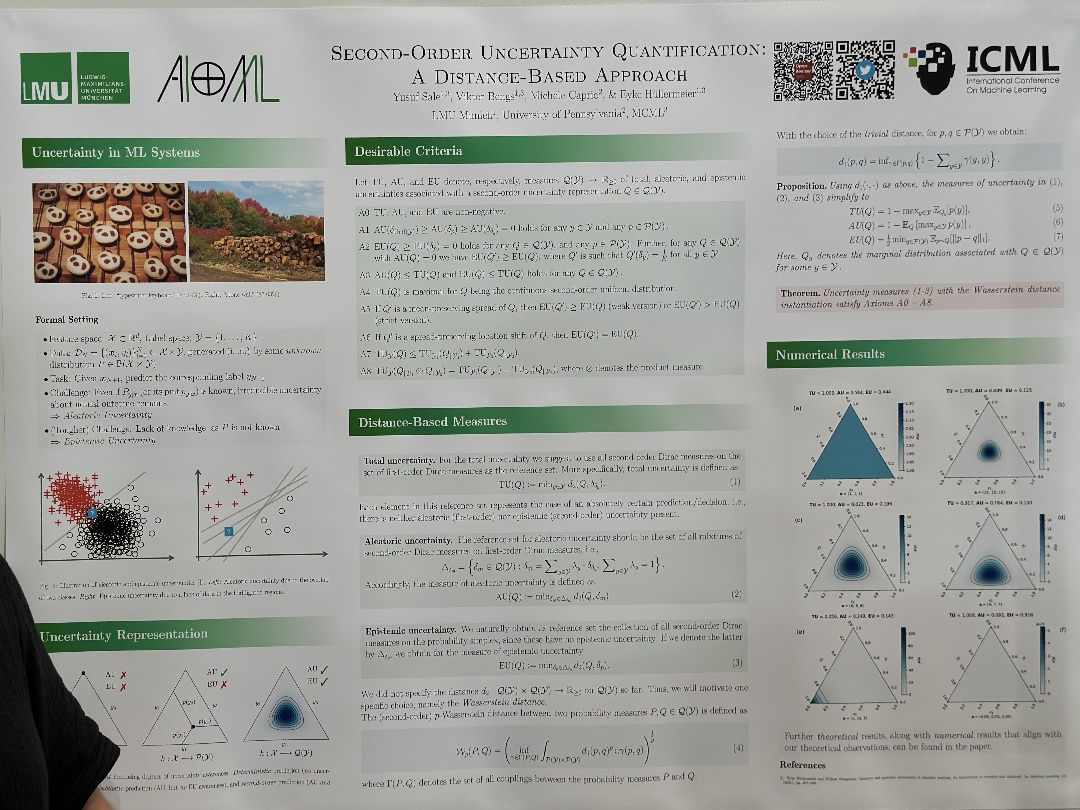
\includegraphics[width=68mm]{out_reduced/IMG_1562.jpeg}} & \textbf{Power{-}Law distributions and Fisher's information measure} 
 \textit{F. Pennini,A. Plastino} 

SECOND{-}ORDER UNCERTAINTY QUANTIFICATION:

\url{http://dx.doi.org/10.1016/j.physa.2003.10.076}\\\raisebox{-\height}{\s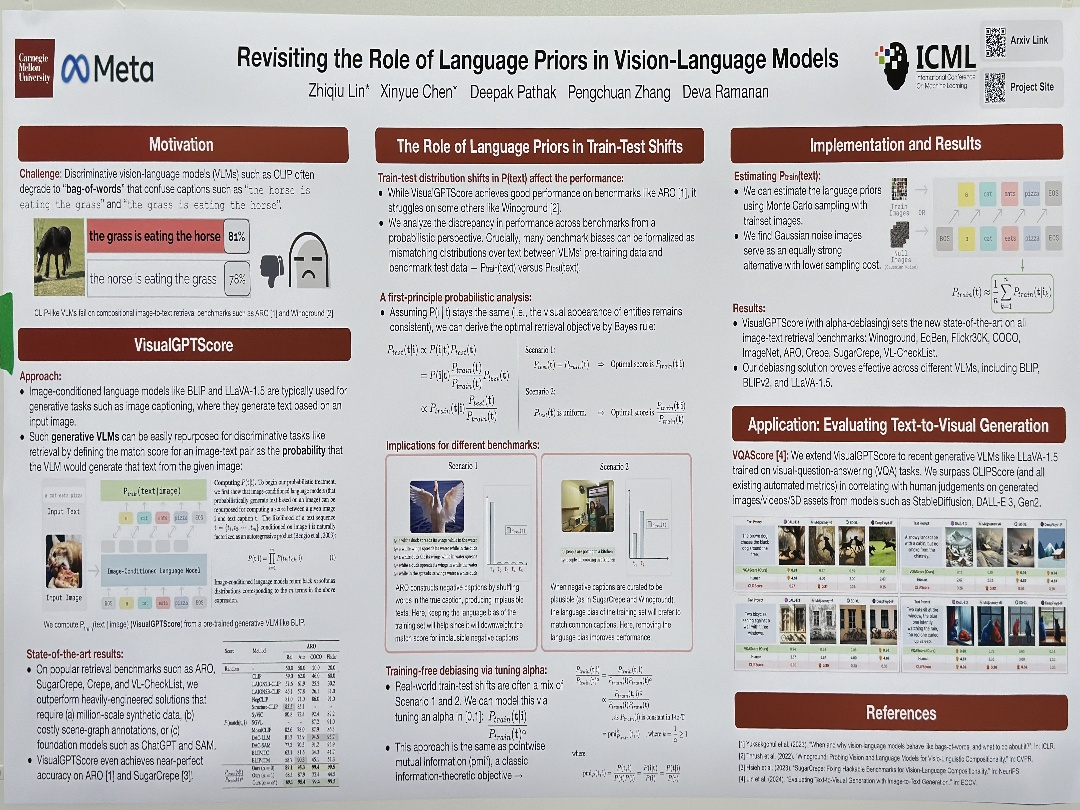
\includegraphics[width=68mm]{out_reduced/IMG_1558.jpeg}} & \textbf{Revisiting the Role of Language Priors in Vision{-}Language Models} 
 \textit{{[}1{]} Yuksekgonul et al. (2023). "When and why vision{-}language models behave like bags{-}of{-}words, and what to do about it?", In: ICLR.} 

Revisiting the Role of Language Priors in Vision{-}Language Models

\url{}\\\raisebox{-\height}{\s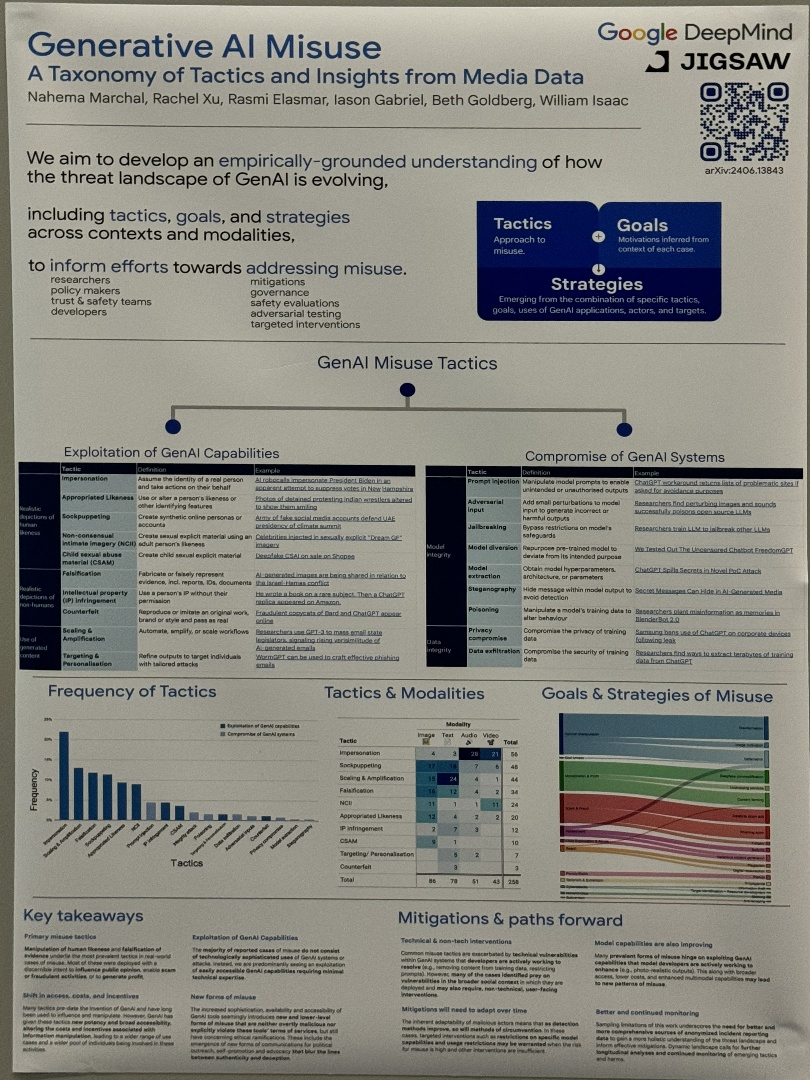
\includegraphics[width=68mm]{out_reduced/IMG_1597.jpeg}} & \textbf{Generative AI Misuse: A Taxonomy of Tactics and Insights from Real{-}World Data} 
 \textit{Nahema Marchal,Rachel Xu,Rasmi Elasmar,Iason Gabriel,Beth Goldberg,William Isaac} 

A Taxonomy of Tactics and Insights from Media Data

\url{http://arxiv.org/abs/2406.13843v2}\\\raisebox{-\height}{\s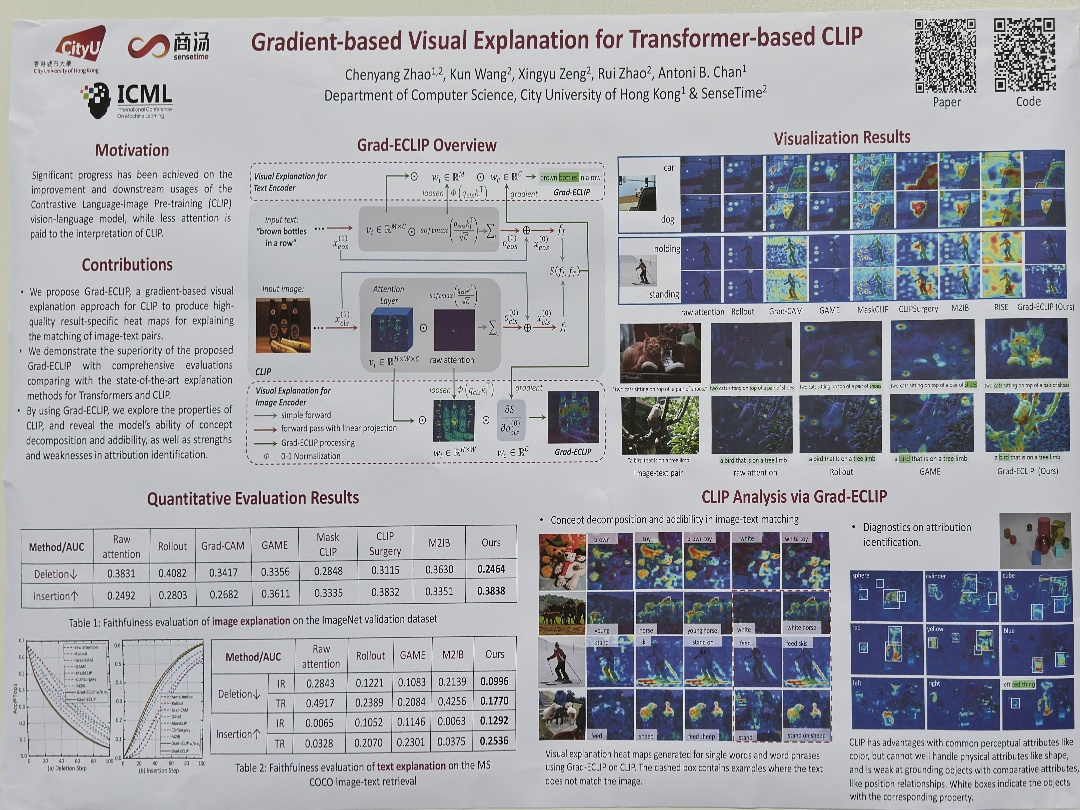
\includegraphics[width=68mm]{out_reduced/IMG_1539.jpeg}} & \textbf{RCA: Region Conditioned Adaptation for Visual Abductive Reasoning} 
 \textit{Hao Zhang,Yeo Keat Ee,Basura Fernando} 

Gradient{-}based Visual Explanation for Transformer{-}based CLIP

\url{http://arxiv.org/abs/2303.10428v4}\\\raisebox{-\height}{\s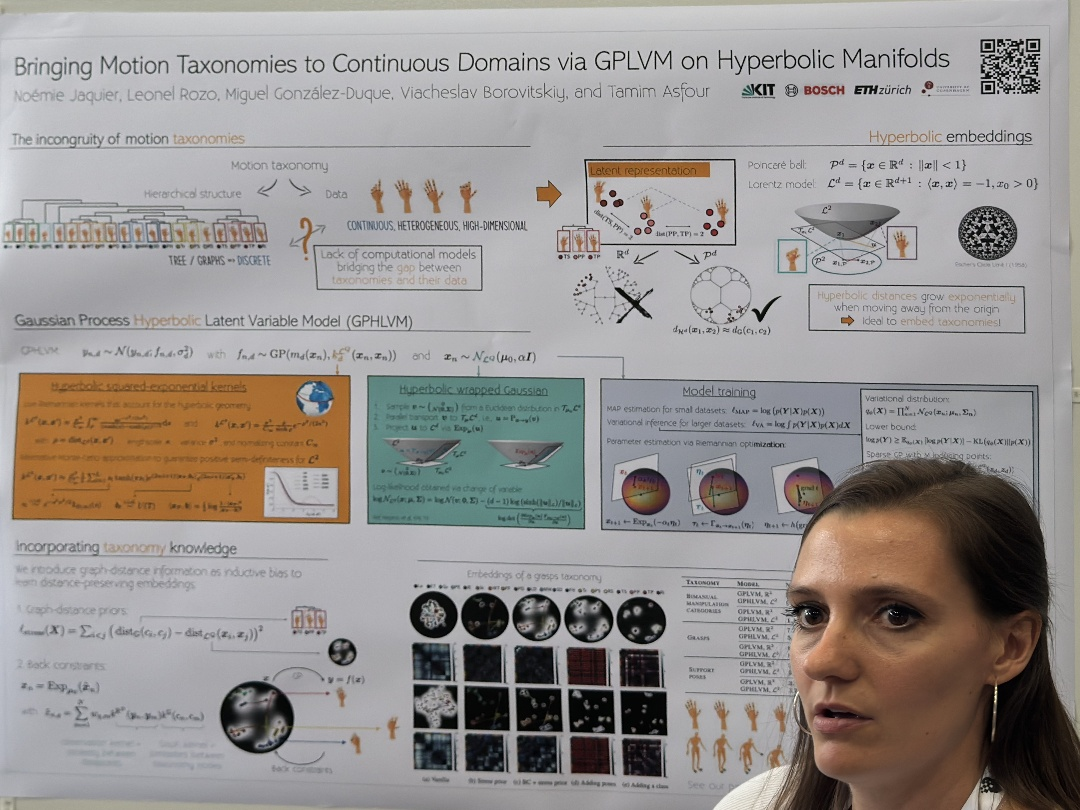
\includegraphics[width=68mm]{out_reduced/IMG_1515.jpeg}} & \textbf{Bringing motion taxonomies to continuous domains via GPLVM on hyperbolic manifolds} 
 \textit{Noémie Jaquier,Leonel Rozo,Miguel González{-}Duque,Viacheslav Borovitskiy,Tamim Asfour} 

Bringing Motion Taxonomies to Continuous Domains via GPLVM on Hyperbolic Manifolds

\url{http://arxiv.org/abs/2210.01672v4}\\\raisebox{-\height}{\s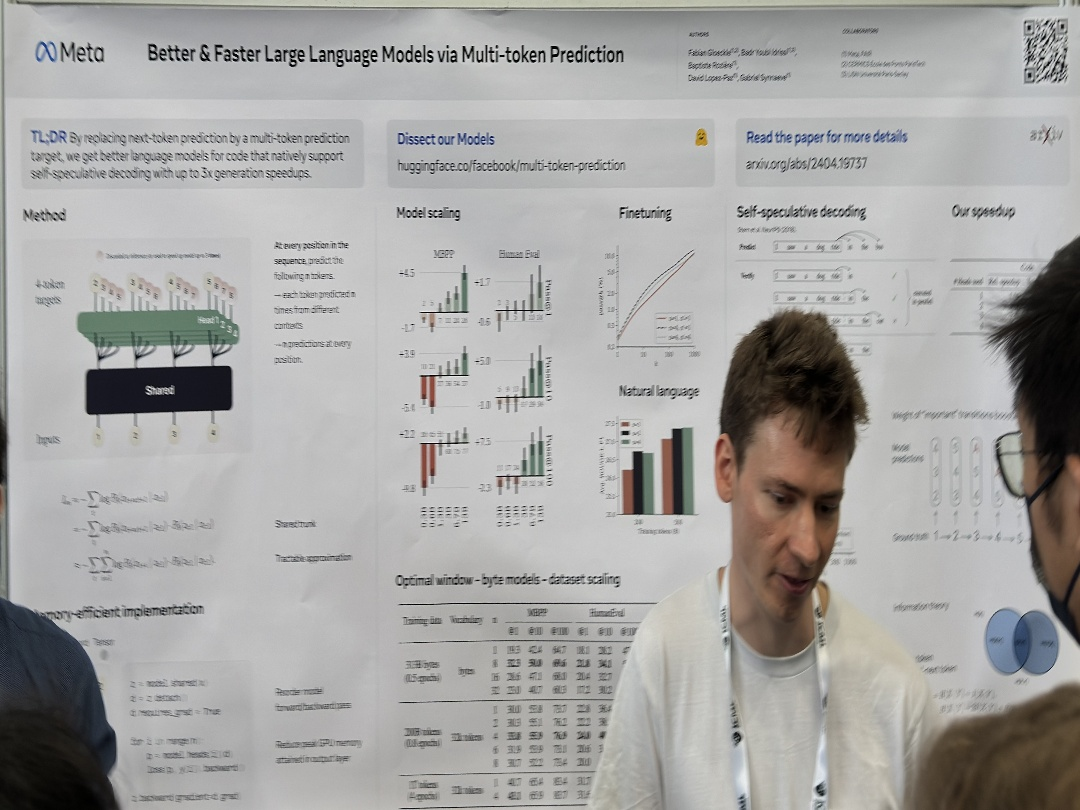
\includegraphics[width=68mm]{out_reduced/IMG_1542.jpeg}} & \textbf{Better \& Faster Large Language Models via Multi{-}token Prediction} 
 \textit{Fabian Gloeckle,Badr Youbi Idrissi,Baptiste Rozière,David Lopez{-}Paz,Gabriel Synnaeve} 

Better \& Faster Large Language Models via Multi{-}token Prediction

\url{http://arxiv.org/abs/2404.19737v1}\\\raisebox{-\height}{\s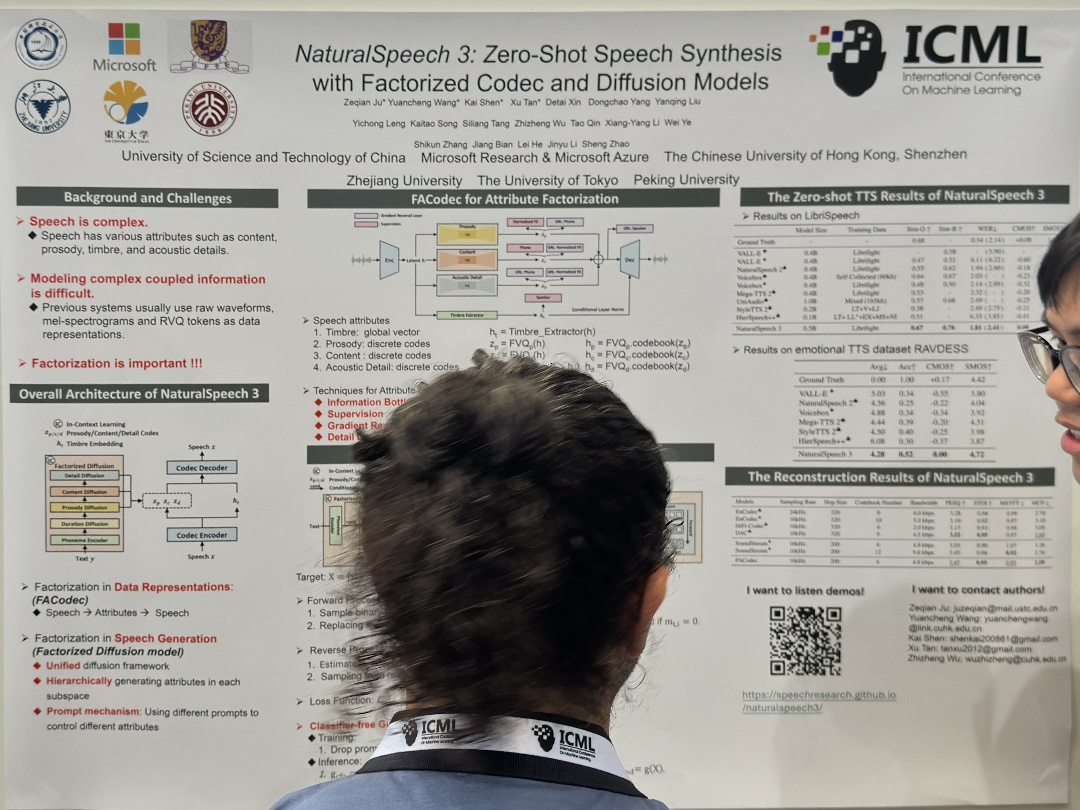
\includegraphics[width=68mm]{out_reduced/IMG_1543.jpeg}} & \textbf{TJ{-}FlyingFish: Design and Implementation of an Aerial{-}Aquatic Quadrotor with Tiltable Propulsion Units} 
 \textit{Xuchen Liu,Minghao Dou,Dongyue Huang,Biao Wang,Jinqiang Cui,Qinyuan Ren,Lihua Dou,Zhi Gao,Jie Chen,Ben M. Chen} 

University of Science and Technology of China Microsoft Research \& Microsoft Azure The Chinese University of Hong Kong, Shenzhen

\url{http://arxiv.org/abs/2301.12344v2}\\\raisebox{-\height}{\s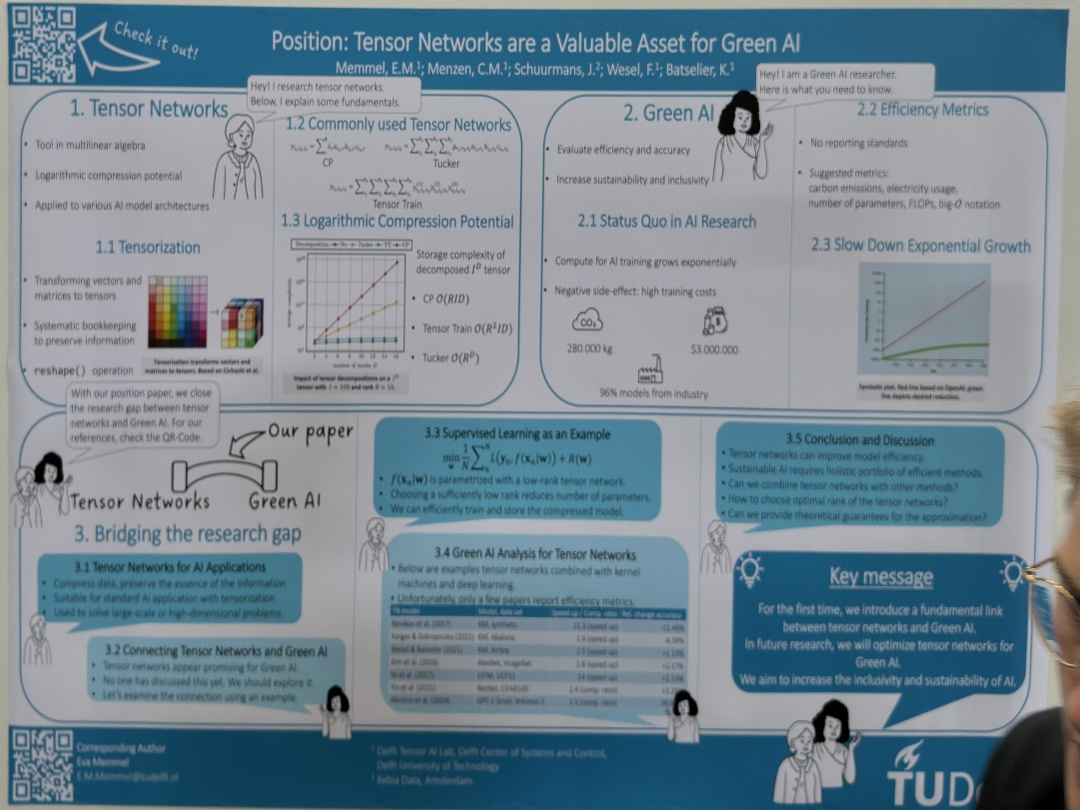
\includegraphics[width=68mm]{out_reduced/IMG_1514.jpeg}} & \textbf{Position: Tensor Networks are a Valuable Asset for Green AI} 
 \textit{Eva Memmel,Clara Menzen,Jetze Schuurmans,Frederiek Wesel,Kim Batselier} 

Position: Tensor Networks are a Valuable Asset for Green Al

\url{http://arxiv.org/abs/2205.12961v2}\\\raisebox{-\height}{\s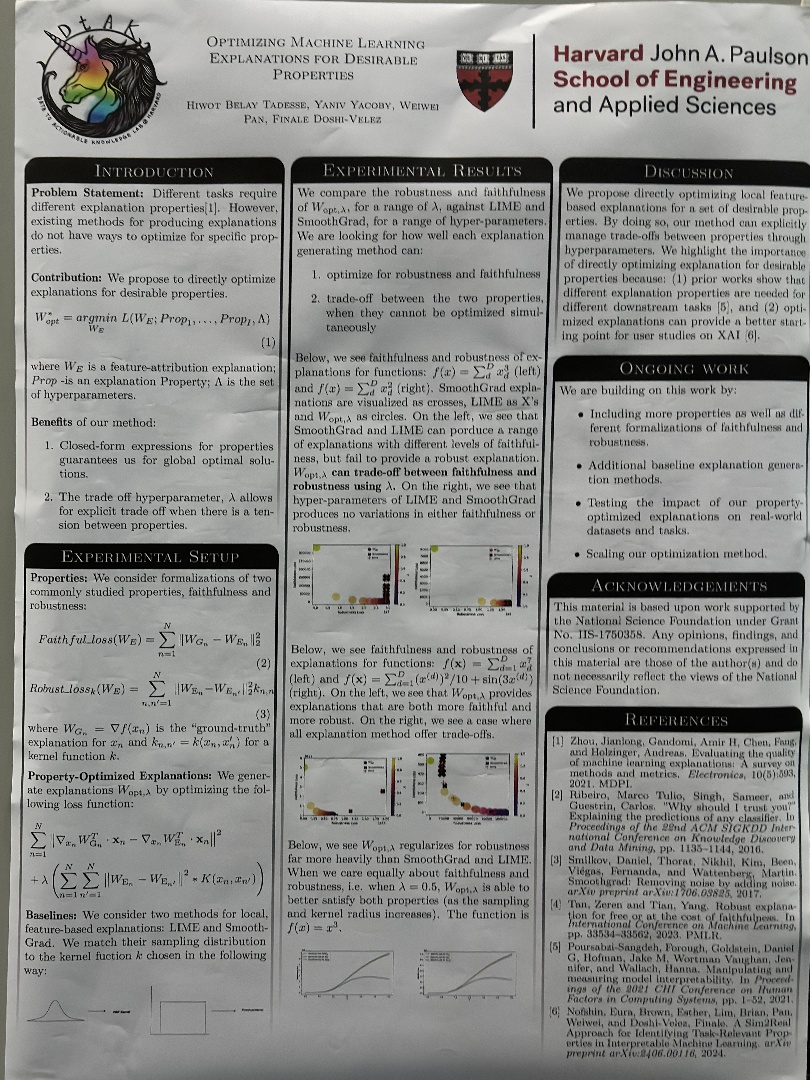
\includegraphics[width=68mm]{out_reduced/IMG_1596.jpeg}} & \textbf{School of Engineering} 
 \textit{{[}1) Zhou, Jianlong, Gandomi, Amir H, Chen, Fang,} 

School of Engineering

\url{}\\\raisebox{-\height}{\s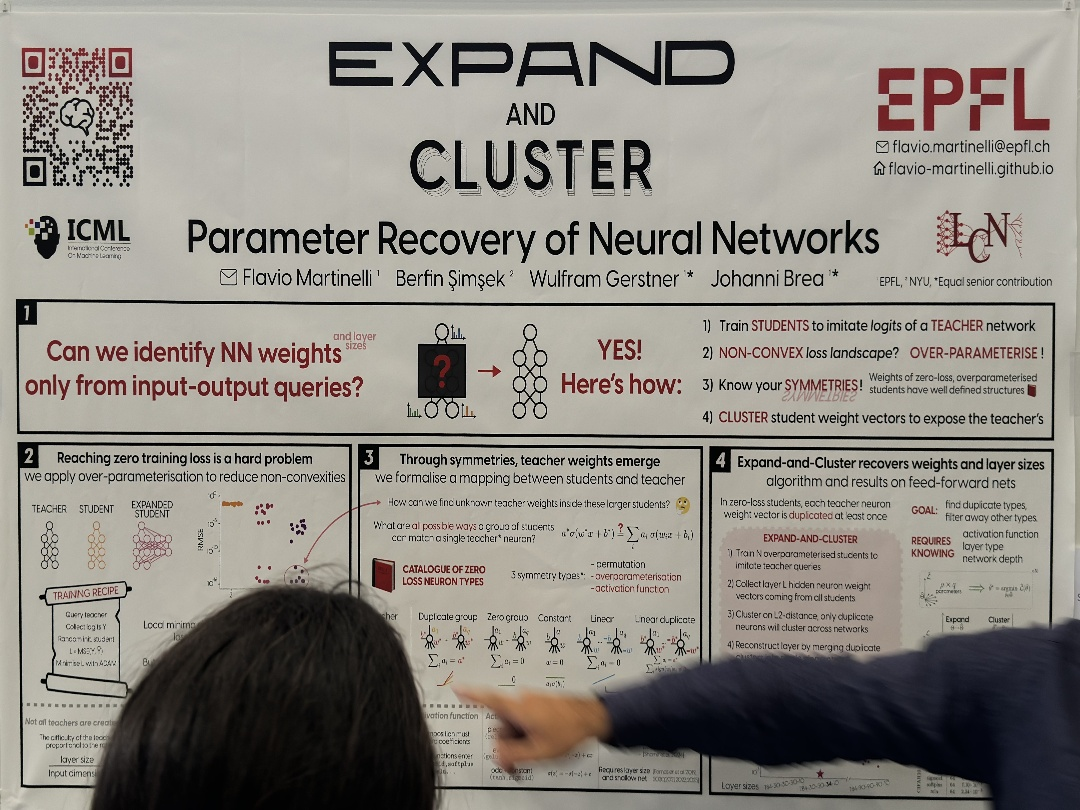
\includegraphics[width=68mm]{out_reduced/IMG_1559.jpeg}} & \textbf{Dual Convexified Convolutional Neural Networks} 
 \textit{Site Bai,Chuyang Ke,Jean Honorio} 

Parameter Recovery of Neural Networks

\url{http://arxiv.org/abs/2205.14056v2}\\\raisebox{-\height}{\s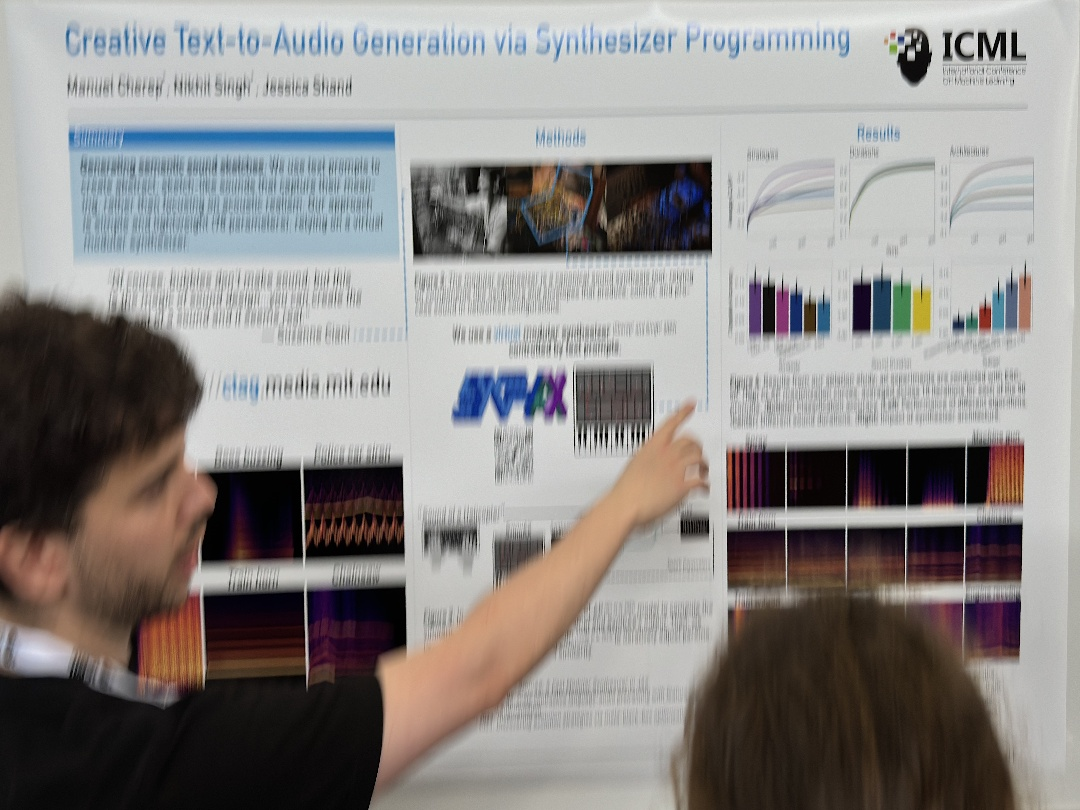
\includegraphics[width=68mm]{out_reduced/IMG_1518.jpeg}} & \textbf{Luban: Building Open{-}Ended Creative Agents via Autonomous Embodied Verification} 
 \textit{Yuxuan Guo,Shaohui Peng,Jiaming Guo,Di Huang,Xishan Zhang,Rui Zhang,Yifan Hao,Ling Li,Zikang Tian,Mingju Gao,Yutai Li,Yiming Gan,Shuai Liang,Zihao Zhang,Zidong Du,Qi Guo,Xing Hu,Yunji Chen} 

Creative Text{-}to{-}Audio Generation Via Synthesizer Programming

\url{http://arxiv.org/abs/2405.15414v1}\\\raisebox{-\height}{\s\includegraphics[width=68mm]{out_reduced/IMG_1534.jpeg}} & \textbf{A Survey on Trustworthy Edge Intelligence: From Security and Reliability To Transparency and Sustainability} 
 \textit{Xiaojie Wang,Beibei Wang,Yu Wu,Zhaolong Ning,Song Guo,Fei Richard Yu} 

TRUSTWORTHY ACTIONABLE PERTURBATIONS

\url{http://arxiv.org/abs/2310.17944v2}\\\raisebox{-\height}{\s\includegraphics[width=68mm]{out_reduced/IMG_1522.jpeg}} & \textbf{Monitoring AI{-}Modified Content at Scale: A Case Study on the Impact of ChatGPT on AI Conference Peer Reviews} 
 \textit{Weixin Liang,Zachary Izzo,Yaohui Zhang,Haley Lepp,Hancheng Cao,Xuandong Zhao,Lingjiao Chen,Haotian Ye,Sheng Liu,Zhi Huang,Daniel A. McFarland,James Y. Zou} 

Monitoring Al{-}Modified Content at Scale:

\url{http://arxiv.org/abs/2403.07183v2}\\\end{longtblr}

\end{document}